\chapter{Eigene Resultate} \label{chap:results}

Die Theorie wird in Kapitel \ref{chap:results} verwendet, um die Resultate zu erläutern.
In diesen werden weitere topologische Indizes, die im theoretischen Teil nicht vorgestellt wurden, analysiert und verglichen.

Für aufschliessende Informationen zu allen aktuellen und bedeutsamen topologischen Indizes können bestehende Literaturwerke der Graphentheorie zurate gezogen werden \cite{dehmer_information_2012,ravi_computation_2022,amin_analysis_2022,sarkar_neighbourhood_2021}.
Der Werdegang der Graphenklassifikation wurde aufgearbeitet und das Thema Graph-Isomorphie erläutert.
Bei der Klassifikation wurden \textit{State-of-the-Art} Methoden und deren Hintergründe vorgestellt.
Als Nächstes folgen die verwendeten Daten für die Resultate sowie der Aufbau der Methodik.

Dieses Kapitel soll einen Überblick über die Resultate dieser Arbeit geben.
Es werden die visualisierten Resultate sowie die Ergebnisse der Tests zusammengefasst.
Die in der Einleitung \ref{chap:introduction} beschriebenen Hypothesen werden getestet und die erwarteten Resultate erarbeitet.

\newpage

\section{Erwartete Resultate}

Im Idealfall wird das Resultat eine quantitative Analyse verschiedener topologischer Indizes sein und einen Beitrag zur Usefulness von topologischen Indizes leisten.
Die quantitative Analyse umfasst eine explorative Datenanalyse der topologischen Indizes in verschiedenen Graph Klassen, eine statistische Analyse der Zusammenhänge zwischen den topologischen Indizes und den Graph-Klassen, so wie eine Machine Learning Analyse der Graph Klassen.

Mit der Analyse sollen die topologischen Indizes auf ihre Sinnhaftigkeit und Anwendbarkeit in verschiedenen Kontexten untersucht werden.
Als Resultat soll eine Auflistung respektive Rangfolge der sinnvollsten Messwerte für die eingegebenen Graphen und topologischen Indizes ausgegeben werden.
Der Algorithmus und die Formel zur Berechnung sollten möglichst einfach zugänglich und variabel sein. Der Code für die Berechnung soll Open Source sein.

Im Schlussteil der Arbeit sollen folgenden Resultate vorliegen:
\begin{itemize}
    \item eine sinnvolle Analyse und Auflistung der topologischen Messwerte,
    \item eine Analyse der Berechnung des Usefulness-Scores von topologischen Indizes in verschiedenen Netzwerkklassen,
    \item ein Python-Modul zur Berechnung des Usefulness-Scores und
    \item Vorschläge von topologischen Messwerten zur Struktur eines gelieferten Netzwerks.
\end{itemize}

Um diese Resultate zu erreichen, werden folgende Schritte durchgeführt:
\begin{enumerate}
    \item Datenaufbereitung,
    \item Durchführung von Experimenten,
    \item Entwicklung eines Systems, welches topologische Indizes sinnvoll vergleicht, sowie
    \item Implementierung der Systeme in Python.
\end{enumerate}

In der folgenden Übersicht ist dargestellt, wie die Erarbeitung der Resultate vonstattengeht:

\begin{figure}[H]
    \centering
    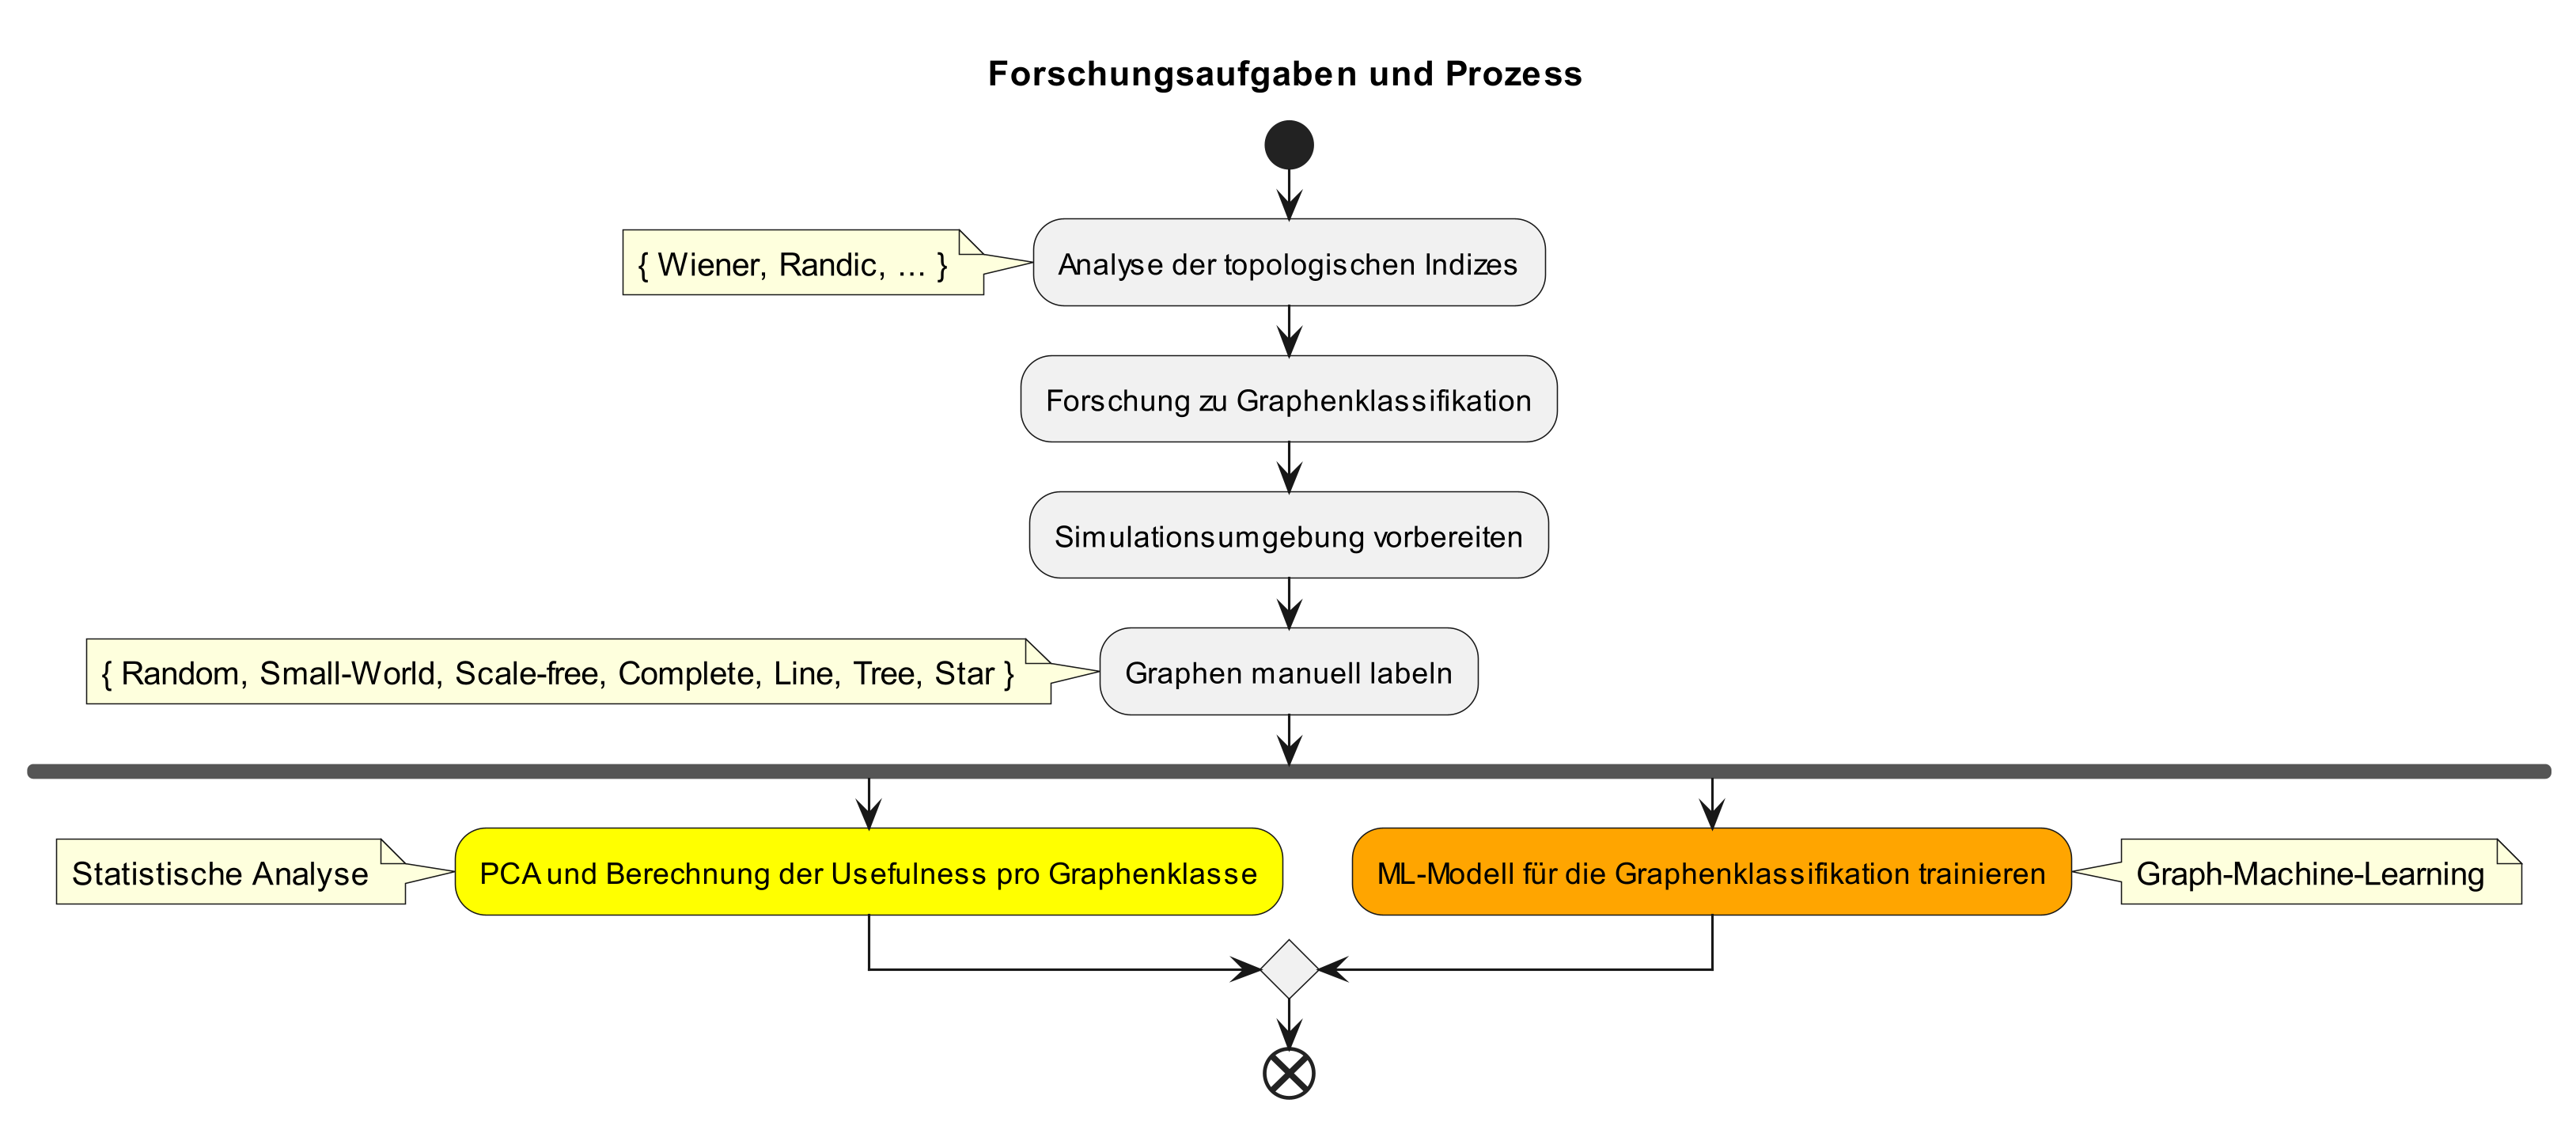
\includegraphics[width=1\textwidth]{images/30_results/activity_research.png}
    \caption{Erarbeitung der Resultate}
    \label{fig:results}
\end{figure}

Auf Abbildung \ref{fig:results} ist dargestellt, auf welchem Weg die Resultate erarbeitet werden. 
Gestartet wird mit der Analyse und Dokumentation der existierenden topologischen Indizes.
Der Studie zur Klassifikation von Graphen folgt das Beschaffen und Klassifizieren der Daten. 
Von da an ist die Arbeit in zwei parallele Arbeitsstränge geteilt. 
Mit einer statistischen Analyse werden die topologischen Indizes miteinander verglichen und daneben wird ein Machine-Learning-Modell entwickelt und trainiert, welches die Graphen klassifiziert. 
Die Resultate der beiden Arbeitsstränge werden zusammengeführt und die Hypothesen getestet.

\newpage

\section{Datenaufbereitung}

\subsection{Simulation}

In der Simulationsumgebung werden diverse Netzwerke mit verschiedenen topologischen Eigenschaften erzeugt und diese gemessen.
Zu Beginn werden verschiedene Netzwerke untersucht, darunter Nauty-Graphen, die aus dem Internet heruntergeladen wurden \cite{mckay_practical_2014}, sowie Netzwerke aus verschiedenen Anwendungsfällen wie biologische, soziale, chemische und Zitat-Netzwerke.

Um die Analyse zu formalisieren, liegt der Fokus der die Arbeit auf formelleren Klassen von Netzwerken.
Dadurch ergeben sich zwei Vorteile für die Analyse:
\begin{itemize}
    \item [+] Die Netzwerke können synthetisch erzeugt werden.
    \item [+] Die Klassen sind formal definiert und in der Literatur gut abgedeckt.
\end{itemize}

Es werden die in der Theorie zu den Netzwerkklassen \ref{sec:graph_classes} definierten Klassen verwendet.
Um Graphen zu generieren, müssen deren Parameter bzw. Eigenschaften dokumentiert werden.
Dadurch werden die Forschungsresultate aus dieser Arbeit reproduzierbar.
Im nächsten Abschnitt werden die genauen Netzstrukturen und ihre Eigenschaften beschrieben.

\newpage

\subsection{Netze und Klassen}

Es folgt das Fundament für die Daten der verwendeten Netzwerke.
Diese sind in verschiedene Klassen eingeteilt.

Die Daten werden eigenständig synthetisch mit Python generiert.
Es handelt sich bei allen Graphen um ungerichtete, zusammenhängende Graphen.

In dieser abgeschlossenen Liste sind die verwendeten Testdaten für die Netzwerkanalyse aufgeführt:

\begin{table}[H]
    \caption{\label{data-table}Alle Graphen, die für die Arbeit generiert wurden und deren Anzahl Knoten.}
    \begin{adjustbox}{minipage=\textwidth, center}
        \scriptsize
        \begin{tabularx}{\textwidth}{|l|X|X|c|}
            \hline
            \textbf{Name} & \textbf{Beschreibung}              & \textbf{Eigenschaften}                                                             & \textbf{Anzahl Graphen} \\
            \hline
            Random        & Random Erdős-Rényi-Graphen         & $ |V| = [5..205] $, \newline $ p = 0.3 $                                            & 1000                     \\
            \hline
            Small-World   & Watts-Strogatz Small-World-Graphen & $ |V| = [5..205] $, \newline $ k-neighbours = \frac{|V|}{2} $, \newline $ p = 0.3 $ & 1000                     \\
            \hline
            Scale-free    & Barabási-Albert-Graphen            & $ |V| = [2..202] $, \newline $ m = \frac{|V|}{2} $                                 & 200                      \\
            \hline
            Complete      & k-reguläre Graphen                & $ |V| = [2..202] $                                                                 & 200                      \\
            \hline
            Line          & Pfadgraphen                       & $ |V| = [2..202] $                                                                 & 200                      \\
            \hline
            Tree          & Bäume (+ Random-Trees)             & $ |V| = [2..11] | [2..202]$                                                          & 400                     \\
            \hline
            Star          & Sterngraphen                      & $ |V| = [2..202] $                                                                 & 200                      \\
            \hline
        \end{tabularx}
    \end{adjustbox}
\end{table}

Um ein besseres Bild der generierten Netze zu ermöglichen, folgt ein visualisiertes Beispiel pro Klasse:

\begin{figure}[H]
    \centering
    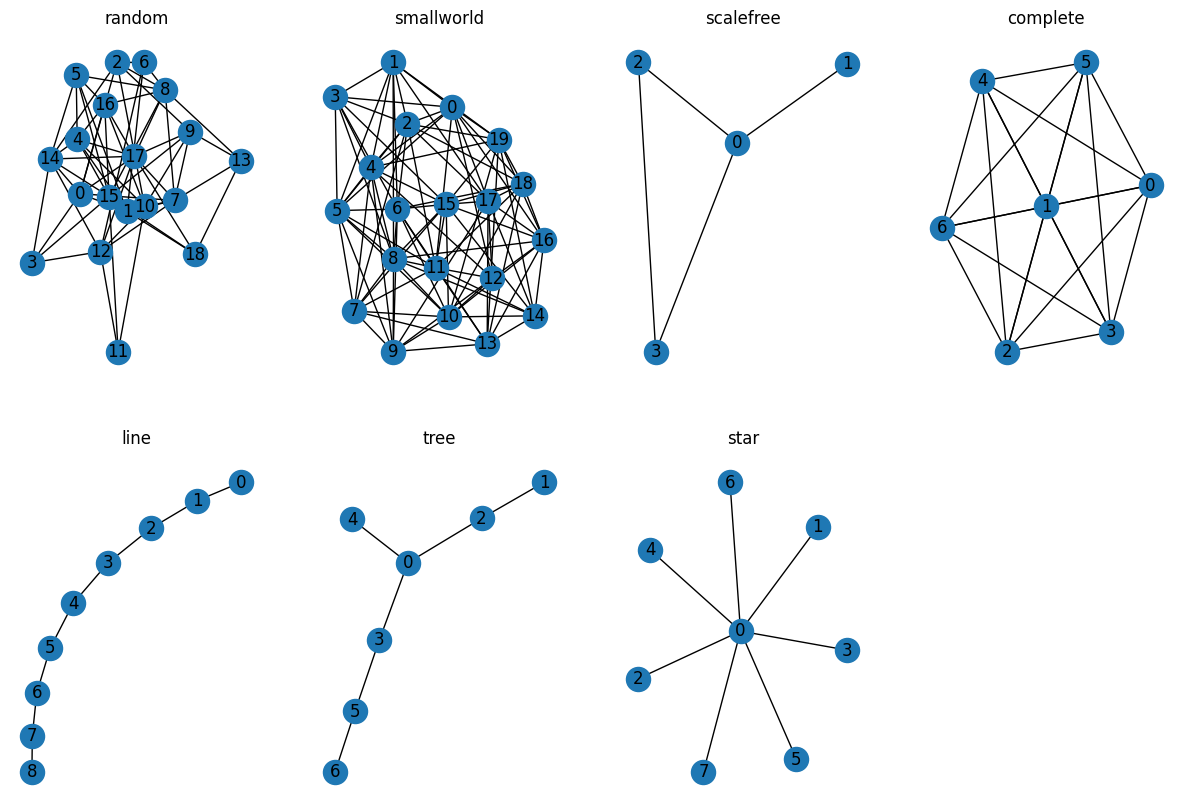
\includegraphics[width=0.6\textwidth]{images/42_data/example_graphs.png}
    \caption{Visualisierung von Graphen mit NetworkX und Matplotlib}
    \label{fig:example_graphs}
\end{figure}

Die Complete, Line-, Tree- und Star-Graphen unterscheiden sich schon bei der ersten Betrachtung stark.
Die Random-Graphen nach Erdős-Rényi und die Small-World-Graphen können auf den ersten Blick ähnlich aussehen, differieren jedoch in der topologischen Struktur, wie bereits in der Theorie erwähnt.

\subsection{Datenaufbereitung und Datenstruktur}

Die Graphen für die Arbeit werden mithilfe von Python und NetworkX erarbeitet \cite{hagberg_exploring_2008}.
Das erstellte Python-Dictionary mit den jeweiligen Graphen ist nachfolgend aufgeführt:

\begin{listing}[H]
    \begin{minted}
        [frame=lines,framesep=2mm,baselinestretch=1.2,bgcolor=LightGray,fontsize=\footnotesize,linenos]
        {python}    
dataset = {
    "random": [],
    "smallworld": [],
    "scalefree": [],
    "complete": [],
    "line": [],
    "tree": [],
    "star": [],
}
    \end{minted}
    \caption{Datenstruktur für die Testdaten}
\end{listing}

In einem nächsten Schritt werden die erstellten Graphen ihrer Klasse zugewiesen, was auch als \emph{Labeling} bezeichnet werden kann. Das Label der Graphen ist der Key des Dictionary.
Diese Labels werden für die spätere Klassifikationsaufgabe verwendet.

\newpage
\section{Vergleich der topologischen Indizes} \label{sec:correlation}

Die Graphen werden zunächst einer explorativen Datenanalyse unterzogen.
Dabei werden erste Zusammenhänge zwischen den topologischen Indizes und den Graphenklassen untersucht.

\subsection{Erste Erkenntnisse und Resultate}

Da es sich um einen mittelgrossen Datensatz handelt und die Knotenanzahl der Graphen generell nicht über 250 liegt, dauert die Berechnung der topologischen Indizes für das ganze Datenset circa 20–30 Minuten.
In der Theorie wurden die relevanten topologischen Indizes für die Analyse der Graphen beschrieben und ausgewählt.
Es gibt eine Vielzahl an Messwerten, die an dieser Stelle verwendet werden könnten.
Die Auswahl der topologischen Indizes ist eine subjektive Entscheidung, die auf der Erfahrung und dem Wissen des Autors basiert.
Später kann die Auswahl der topologischen Indizes erweitert werden, da der Code als parametrierbares, wiederverwendbares Modul entwickelt wird.
Es werden folgende topologische Indizes untersucht:

\begin{table}[H]
    \caption{Topologische Indizes unter Betrachtung}
    \begin{adjustbox}{minipage=\textwidth, center}
        \scriptsize
        \begin{tabularx}{\textwidth}{|l|X|c|}
            \hline
            \textbf{Name}                     & \textbf{Beschreibung}                                                                                                                                                                                                                                    & \textbf{Implementierung} \\
            \hline
            \textbf{Wiener-Index}             & Summe aller kürzesten Pfadlängen zwischen allen Paaren von Knoten in einem Graphen                                                                                                                                                                       & \textit{grinpy}          \\
            \hline
            \textbf{Randic-Index}             & Summe der Wurzel der Gradzahlen aller Knoten in einem Graphen                                                                                                                                                                                            & \textit{grinpy}          \\
            \hline
            \textbf{Generalized Randić-Index} & Erweiterung des Randić-Index, die nicht nur die Knotengrade berücksichtigt, sondern auch andere topologische Informationen wie die Distanz zwischen Knoten, um eine umfassendere Charakterisierung der topologischen Struktur von Graphen zu ermöglichen & \textit{grinpy}          \\
            \hline
            \textbf{Harmonic-Index}           & Harmonische Zentralität in Netzwerken, die als Summe der inversen harmonischen Mittelwerte aller kürzesten Pfadlängen zwischen jedem Knoten und allen anderen Knoten im Netzwerk definiert ist.                                                          & \textit{grinpy}          \\
            \hline
            \textbf{ABC-Index}                & Mass für die Konnektivität von Knoten in Graphen, definiert als Summe der Produkte aus den Gradzahlen der beteiligten Knoten und der Anzahl der Kanten zwischen ihnen                                                                                    & \textit{grinpy}          \\
            \hline
            \textbf{First Zagreb-Index}       & Summe der Quadrate der Gradzahlen aller Knoten in einem Graphen                                                                                                                                                                                          & \textit{grinpy}          \\
            \hline
            \textbf{Second Zagreb-Index}      & Summe der Produkte der Gradzahlen von Paaren benachbarter Knoten                                                                                                                                                                                         & \textit{grinpy}          \\
            \hline
            \textbf{Estrada-Index}            & Summe der Eigenwerte des Netzwerk-Adjazenzmatrix-Exponenten                                                                                                                                                                                              & \textit{networkx}        \\
            \hline
            \textbf{Hosoya-Z-Index}           & Summe von einer Menge an Zahlen $(p(G,k))$, welche die Anzahl der Möglichkeiten angibt, wie $k$ Bindungen aus $G$ so ausgewählt werden, dass keine von ihnen miteinander verbunden sind                                                                  & \textit{Eigenes Werk}    \\
            \hline
            \textbf{CII}                      & Summe der Entropien der Knotenfarben des minimalen färbenden Schemas eines Graphen                                                                                                                                                                       & \textit{Eigenes Werk}    \\
            \hline
            \textbf{Szeged-Index}             & Summe der Produkte von Graden benachbarter Knoten                                                                                                                                                                                                        & \textit{Eigenes Werk}    \\
            \hline
        \end{tabularx}
    \end{adjustbox}
\end{table}

\subsubsection{Berechnung der Indizes}

Nachdem die Graphen vorbereitet und eingelesen sind, werden die Indizes berechnet.
Ein Teil dieser Berechnung erfolgt mithilfe der NetworkX-Bibliothek \cite{hagberg_exploring_2008}, wobei die GrinPy-Bibliothek in Kombination mit NetworkX genutzt wird \cite{amos_grinpy_2022}, wie zuvor erwähnt.

Um die Indizes effizient berechnen zu können, wird das Dictionary von Graphen pro Klasse durchgearbeitet, die Indizes werden berechnet und in einem Dictionary abgespeichert.
Um die Variablen in einem späteren Schritt wiederverwenden zu können, wird das Dictionary in einer JSON-Datei gespeichert.
Der Key der Werte ist der Index des Graphen, zum Beispiel \mintinline{text}{line_1} aus der eingelesenen Graphenliste.
Die Werte des Dictionary sind die berechneten Indizes.

\begin{listing}[H]
    \begin{minted}
        [frame=lines,framesep=2mm,baselinestretch=1.2,bgcolor=LightGray,fontsize=\footnotesize,linenos,breaklines]
        {python}   
import grinpy as gp
from indices import indices

def get_topological_indices(G):
    ''' Create a dictionary with the topological indices of a graph G.'''
    topological_indices = {}
    topological_indices['nodes'] = nx.number_of_nodes(G)
    topological_indices['wiener_index'] = gp.wiener_index(G)
    topological_indices['randic_index'] = gp.randic_index(G)
    topological_indices['generalized_randic_index'] = gp.generalized_randic_index(G, 2)
    topological_indices['harmonic_index'] = gp.harmonic_index(G)
    topological_indices['atom_bond_connectivity_index'] = gp.atom_bond_connectivity_index(G)
    topological_indices['first_zagreb_index'] = gp.first_zagreb_index(G)
    topological_indices['second_zagreb_index'] = gp.second_zagreb_index(G)
    topological_indices['estrada_index'] = nx.estrada_index(G)
    topological_indices['hosoya_z_index'] = indices.hosoya_z_index(G)
    topological_indices['chromatic_information_index'] = indices.chromatic_information_index(G)
    topological_indices['szeged_index'] = indices.szeged_index(G)

    return topological_indices
    \end{minted}
    \caption{Diese Funktion berechnet die topologischen Indizes für einen Graphen.}
    \label{lst:indices}
\end{listing}

Wie in der Tabelle der zu untersuchenden topologischen Indizes \ref{data-table} zu sehen ist, werden einige Berechnungen aus der Bibliothek \mintinline{python3}{GrinPy} verwendet. Andere, wie  der Hosoya-Z-Index, werden in einem eigenen \mintinline{python3}{Indices}-Modul implementiert.

\subsubsection{Explorative Datenanalyse und erste Visualisierung}

Nachdem die Indizes berechnet sind, werden die Daten visualisiert. Die Matplotlib-Bibliothek wird für die Visualisierung verwendet \cite{Hunter:2007}.

Um den Vergleich von zwei oder mehr Indizes sinnvoll zu gestalten, werden die Daten normalisiert und standardisiert.

Ein möglicher Vergleich von Graphen besteht darin, die Indizes innerhalb einer Klasse von Graphen einander gegenüberzustellen. Hierbei wird der Index des Graphen auf der x-Achse und der entsprechende Index-Wert auf der y-Achse dargestellt. Der Index des Graphen entspricht dem Key des zugrundeliegenden Dictionary.

Beispielsweise werden in der folgenden Analyse der Randić-Index und der generalisierte Randić-Index verglichen. Die Graphen für den Vergleich werden aus allen nicht isomorphen Graphen bis zu einer Grösse von 10 Knoten aus Nauty ausgewählt.

\begin{figure}[H]
    \centering
    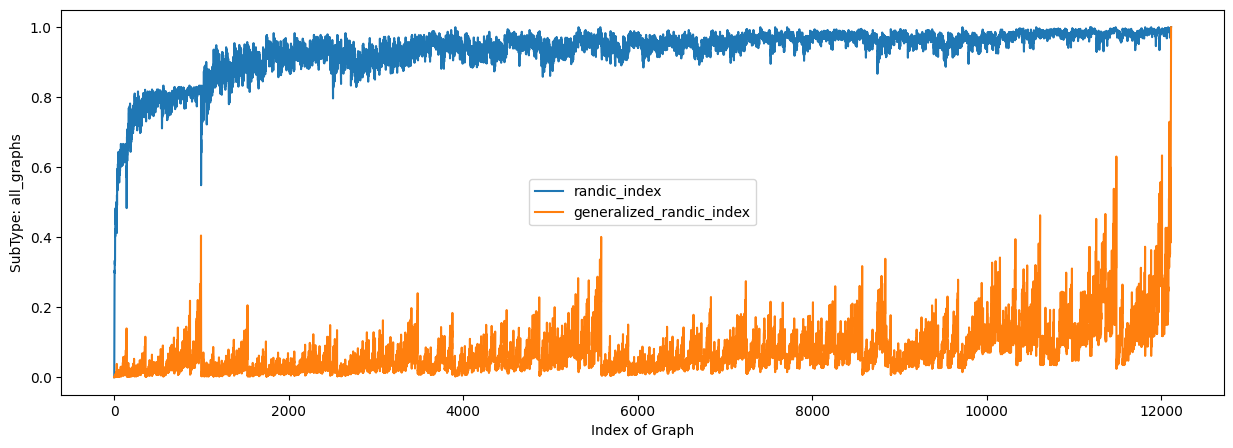
\includegraphics[width=9cm]{images/42_data/explorative_analysis_nauty.png}
    \caption{Vergleich des normalisierten Randić- und des generalisierten Randić-Index von allen non isomorphic graphs (Nauty) bis 10 Knoten}
    \label{fig:explorative_analysis}
\end{figure}


\subsection{Vergleich der topologischen Indizes}

Es werden alle topologischen Indizes, für alle Graphen berechnet, auf die Klassen aufgeteilt und normalisiert.
Die Normalisierung erfolgt durch die Methode \mintinline{python3}{StandardScaler} aus \mintinline{python3}{scikit-learn} mit $ z = (x-u) / s $.
Dabei ist $u$ der Mittelwert und $s$ die Standardabweichung der Werte.

Danach werden die Werte der topologischen Indizes auf der y-Achse und die Anzahl Knoten der Graphen auf der x-Achse visualisiert.

\noindent\hrulefill\par
\noindent\makebox[\textwidth][c]{%
    \begin{minipage}{\textwidth}
        \begin{figure}[H]
            \begin{subfigure}{.45\textwidth}
                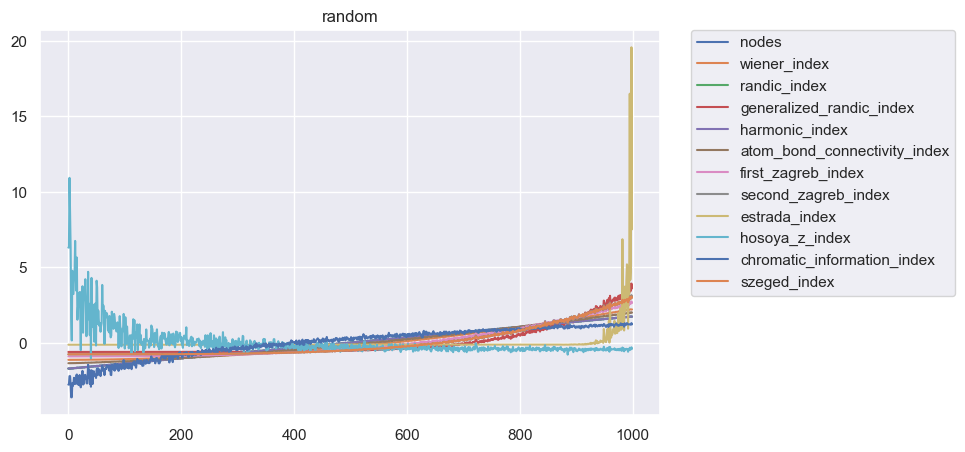
\includegraphics[width=\textwidth]{images/30_results/random-ti-comparison.png}
                \caption{Topologische Indizes der Klasse \mintinline{python3}{Random}}
                \label{fig:ti-comparison-random}
            \end{subfigure}%
            \hspace*{\fill}
            \begin{subfigure}{.45\textwidth}
                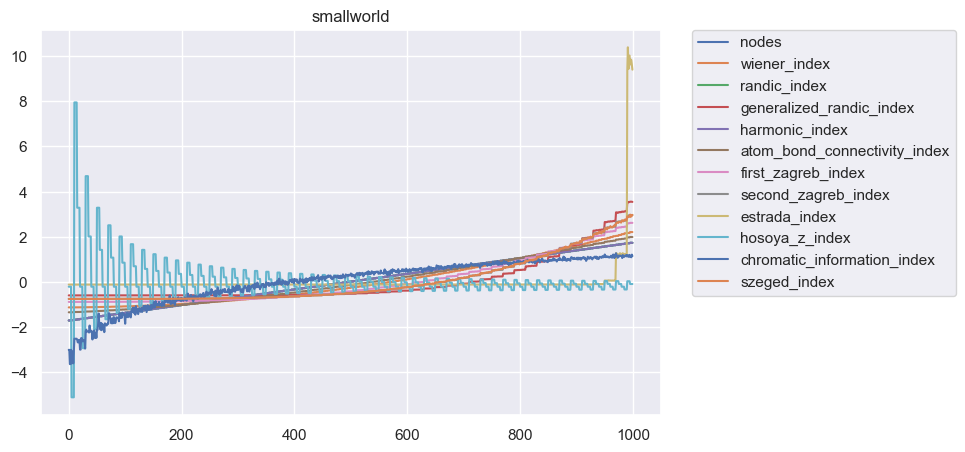
\includegraphics[width=\textwidth]{images/30_results/smallworld-ti-comparison.png}
                \caption{Topologische Indizes der Klasse \mintinline{python3}{Small-World}}
                \label{fig:ti-comparison-smallworld}
            \end{subfigure}

            \begin{subfigure}{.45\textwidth}
                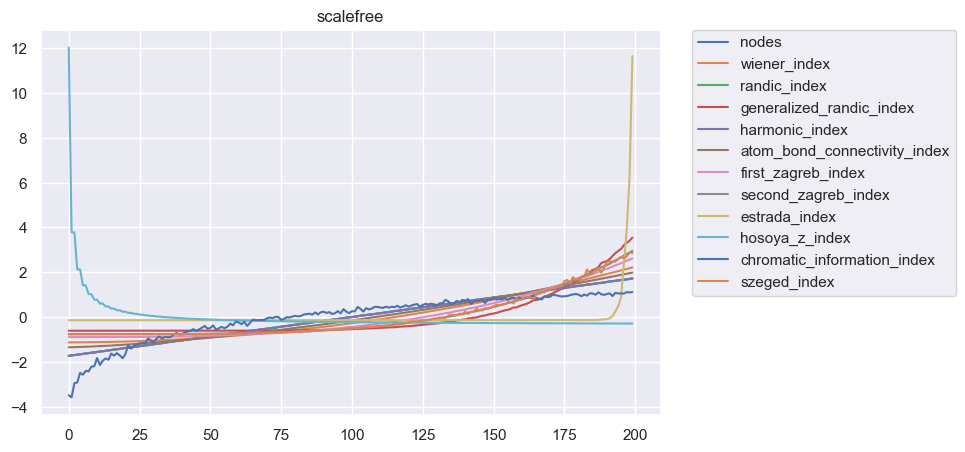
\includegraphics[width=\textwidth]{images/30_results/scalefree-ti-comparison.png}
                \caption{Topologische Indizes der Klasse \mintinline{python3}{Scale-free}}
                \label{fig:ti-comparison-scalefree}
            \end{subfigure}%
            \hspace*{\fill}
            \begin{subfigure}{.45\textwidth}
                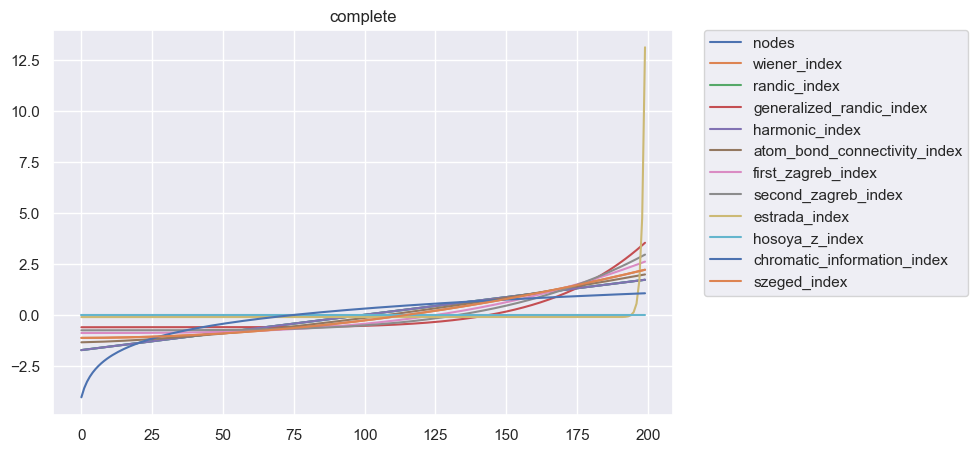
\includegraphics[width=\textwidth]{images/30_results/complete-ti-comparison.png}
                \caption{Topologische Indizes der Klasse \mintinline{python3}{Complete}}
                \label{fig:ti-comparison-complete}
            \end{subfigure}

            \begin{subfigure}{.45\textwidth}
                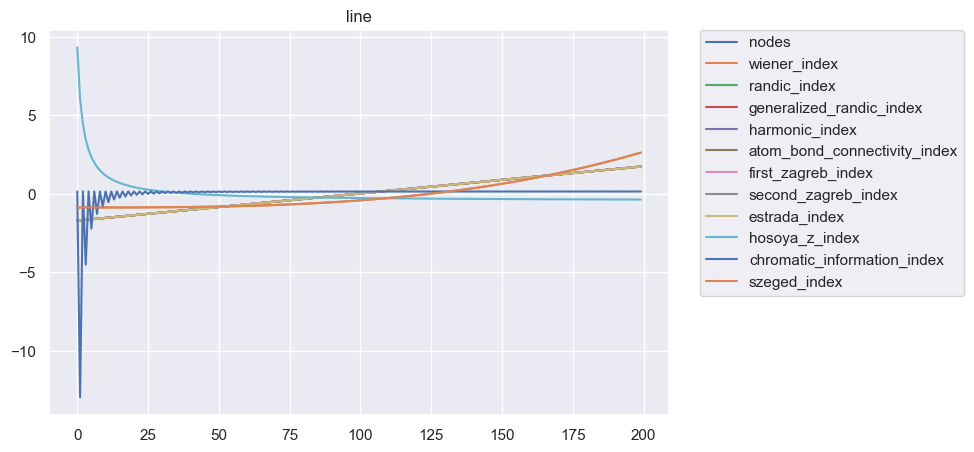
\includegraphics[width=\textwidth]{images/30_results/line-ti-comparison.png}
                \caption{Topologische Indizes der Klasse \mintinline{python3}{Line}}
                \label{fig:ti-comparison-line}
            \end{subfigure}%
            \hspace*{\fill}
            \begin{subfigure}{.45\textwidth}
                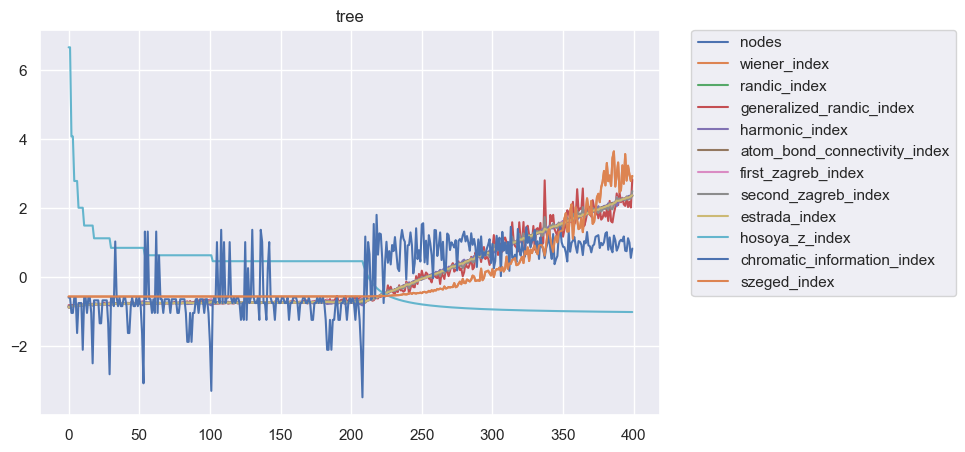
\includegraphics[width=\textwidth]{images/30_results/tree-ti-comparison.png}
                \caption{Topologische Indizes der Klasse \mintinline{python3}{Tree}}
                \label{fig:ti-comparison-tree}
            \end{subfigure}

            \center
            \begin{subfigure}{.45\textwidth}
                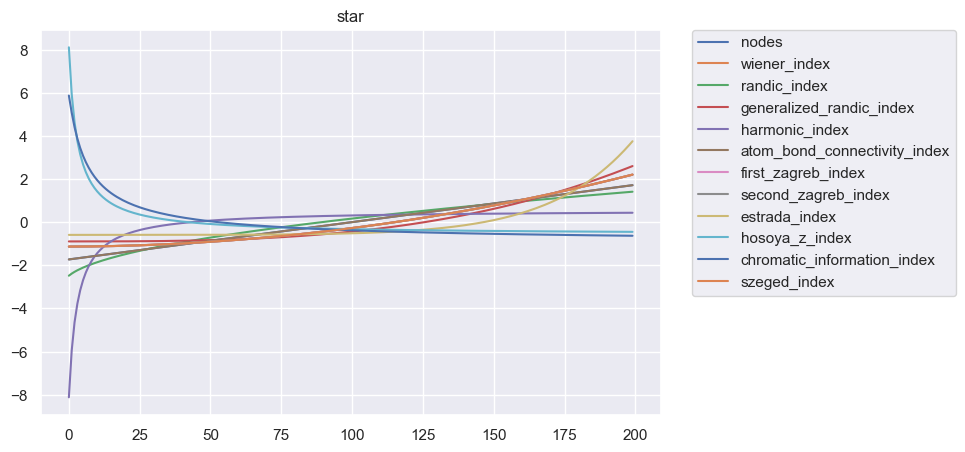
\includegraphics[width=\textwidth]{images/30_results/star-ti-comparison.png}
                \caption{Topologische Indizes der Klasse \mintinline{python3}{Star}}
                \label{fig:ti-comparison-star}
            \end{subfigure}
        \end{figure}
    \end{minipage}}

Die Abbildungen \ref{fig:ti-comparison-random} bis \ref{fig:ti-comparison-star} erhalten die normalisierten topologischen Indizes der verschiedenen Graphenklassen.
Die Resultate sind in Anhang \ref{sec:compare-ti-classes} zur besseren Lesbarkeit in grösser Form zu finden.
Bereits auf den Abbildungen ist zu erkennen, dass sich die topologischen Indizes der Graphenklassen unterscheiden. Es gibt starke Differenzen zwischen den Graphenklassen \mintinline{python3}{Random} und \mintinline{python3}{Small-World} sowie \mintinline{python3}{Scale-free} und \mintinline{python3}{Complete}.

Besonders auffallend sind die Werte der \mintinline{python3}{Tree} und \mintinline{python3}{Small-World} Klassen auf Abbildung \ref{fig:ti-comparison-tree} und \ref{fig:ti-comparison-smallworld}. Hier stechen besonders der Hosoya-Z-Index und der CII heraus, sie besitzen eine besonders hohe Varianz. Sie sind besonders sensitiv auf die Struktur der Graphenklassen bei Änderungen der Knotenzahl \cite{furtula_structure-sensitivity_2013}.

\newpage
\subsection{Korrelation der topologischen Indizes}

Um die Korrelation der topologischen Indizes zu untersuchen, werden die berechneten topologischen Indizes in einer Matrix gespeichert.
Dann werden die Korrelationsmatrizen der topologischen Indizes berechnet und in einer Heatmap geplottet.
Für die Korrelation wird die Spearman-Korrelation \cite{spearman_proof_1904} verwendet.

Diese weist, wie die Pearson-Korrelation, der Korrelation von zwei Variablen einen Wert zwischen -1 und 1 zu. Dabei ist -1 eine vollständige negative Korrelation, 0 bedeutet vollständige unkorrelierte Variablen und 1 eine vollständige positive Korrelation. Die Spearman-Korrelation ist Ausreissern gegenüber weniger empfindlich als die Pearson-Korrelation \cite[p.~73ff]{bartl_statistik_2017}.

In Anhang \ref{sec:correlation-pairs} werden zusätzlich zu den Heatmaps die einzelnen Werte in einem 2D-Scatterplot visualisiert miteinander verglichen. Um die topologischen Indizes besser zu verstehen, wurde entschieden, die topologischen Indizes für eine Klasse auch einzeln zu vergleichen.
Dazu folgen als Nächstes die Zusammenhänge aller topologischen Indizes untereinander.

\begin{figure}[H]
    \centering
    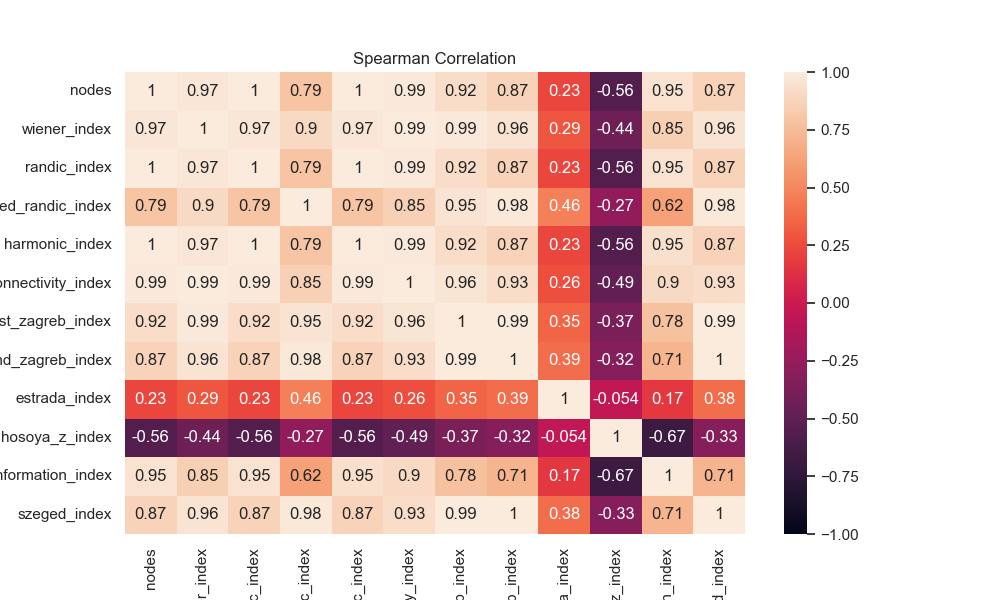
\includegraphics[width=0.8\textwidth]{images/30_results/random-correlation.png}
    \caption{Spearman-Korrelation der topologischen Indizes der Klasse \mintinline{python3}{Random}}
    \label{fig:correlation-random}
\end{figure}

Anhand von Abbildung \ref{fig:correlation-random} kann festgestellt werden, dass zwei topologische Indizes einen fast unkorrelierten Zusammenhang haben. Es handelt sich dabei um die des Estrada-Index und des Hosoya-Z-Index. Ihre Werte liegen zwischen $ -0.67 $ und $ 0.45 $, wobei die meisten Werte nahe um $ 0 $ sind.

Ebenfalls auffallend ist, dass alle anderen topologischen Indizes eine positive Korrelation aufweisen. Auch wenn diese nicht überall besonders hoch ist, ist sie trotzdem generell positiv.

\begin{figure}[H]
    \centering
    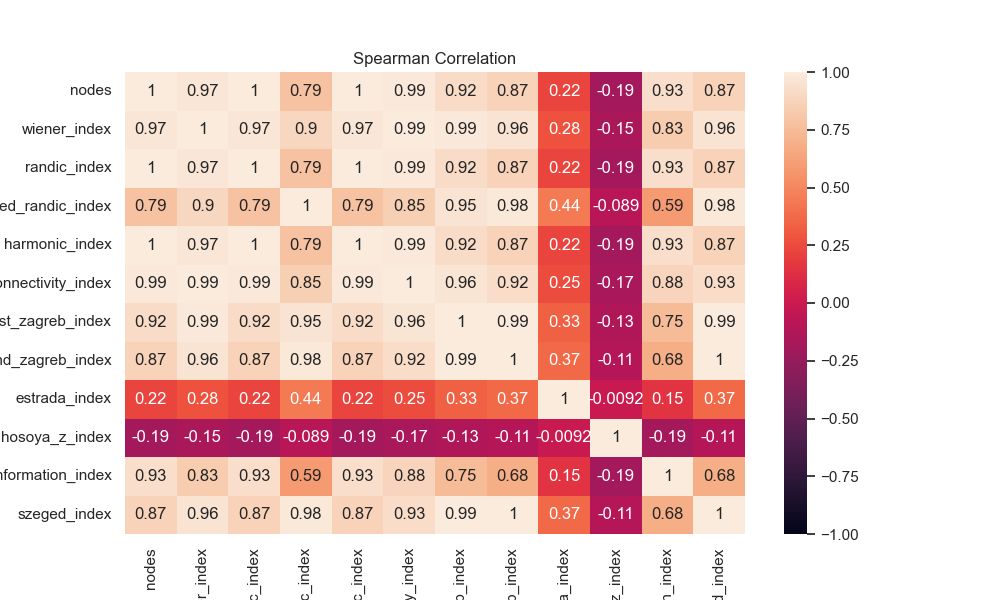
\includegraphics[width=0.8\textwidth]{images/30_results/smallworld-correlation.png}
    \caption{Spearman-Korrelation der topologischen Indizes der Klasse \mintinline{python3}{Small-World}}
    \label{fig:correlation-smallworld}
\end{figure}

\begin{figure}[H]
    \centering
    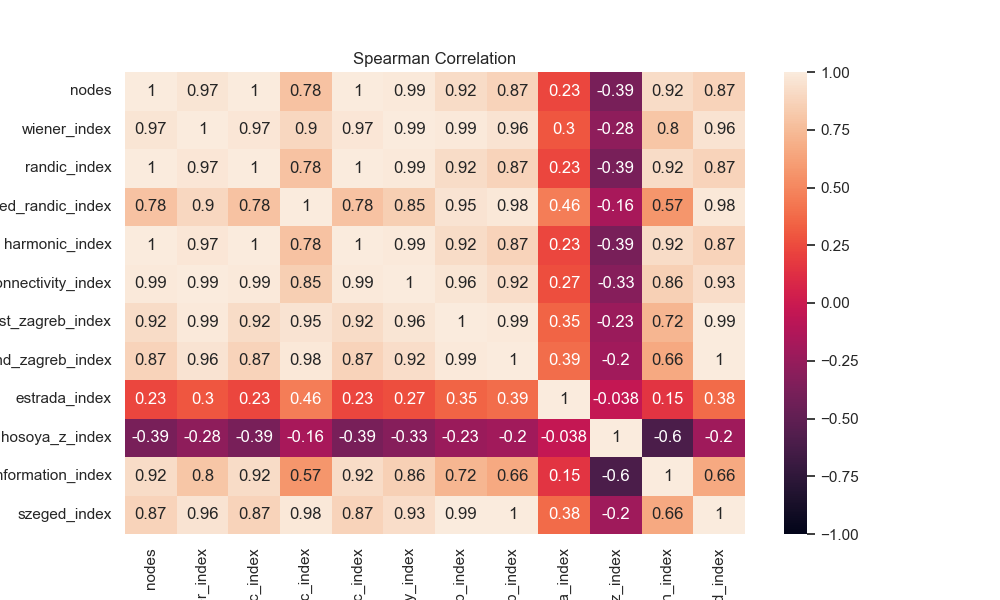
\includegraphics[width=0.8\textwidth]{images/30_results/scalefree-correlation.png}
    \caption{Spearman-Korrelation der topologischen Indizes der Klasse \mintinline{python3}{Scale-free}}
    \label{fig:correlation-scalefree}
\end{figure}

Die Spearman-Korrelation für die Random-Graphen nach Erdős-Rényi, die Small-World-Graphen nach Watts-Strogatz und die Scale-free-Graphen nach Barabási-Albert sind auf den ersten Blick fast identisch. Ihre Heatplots liefern fast identische Ergebnisse.

Die Korrelation des Estrada- und die des Hosoya-Z-Index sind bei den Small-World- und Scale-free-Klassen noch näher bei $ 0 $ als bei den Erdős-Rényi-Graphen.

\begin{figure}[H]
    \centering
    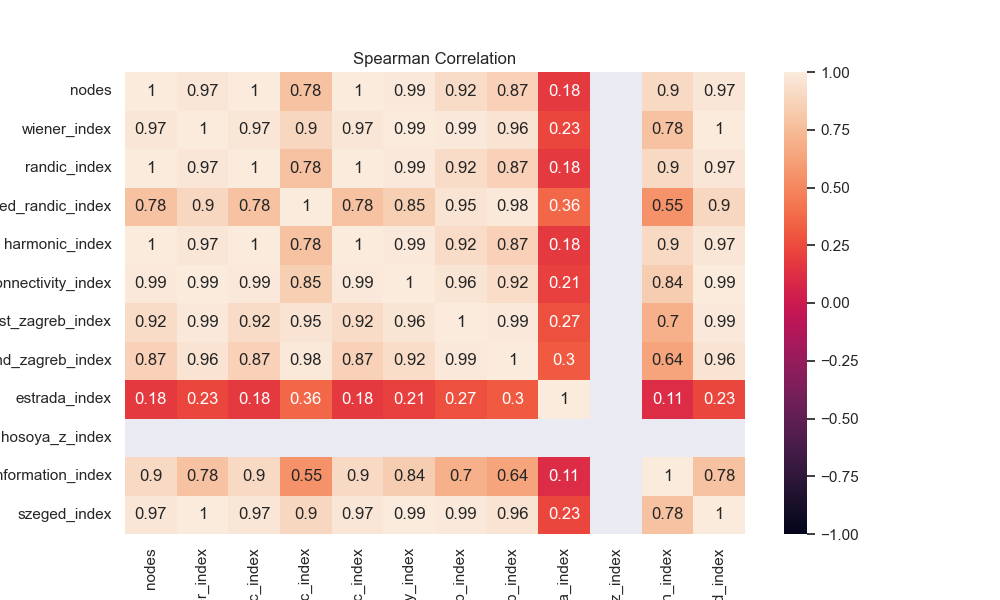
\includegraphics[width=0.7\textwidth]{images/30_results/complete-correlation.png}
    \caption{Spearman-Korrelation der topologischen Indizes der Klasse \mintinline{python3}{Complete}}
    \label{fig:correlation-complete}
\end{figure}

Die Complete-Graphen liefern eine besondere Korrelation. Der Hosoya-Z-Index ist, wie in der Theorie \ref{sec:hosoya_index} beschrieben, bei den Complete-Graphen immer das Maximum.
Neben dem Estrada-Index, welcher ebenfalls wieder nahe bei $ 0 $ liegt, fällt der Szeged-Index auf. Dieser korreliert im Durchschnitt am stärksten mit den anderen topologischen Indizes.

\begin{figure}[H]
    \centering
    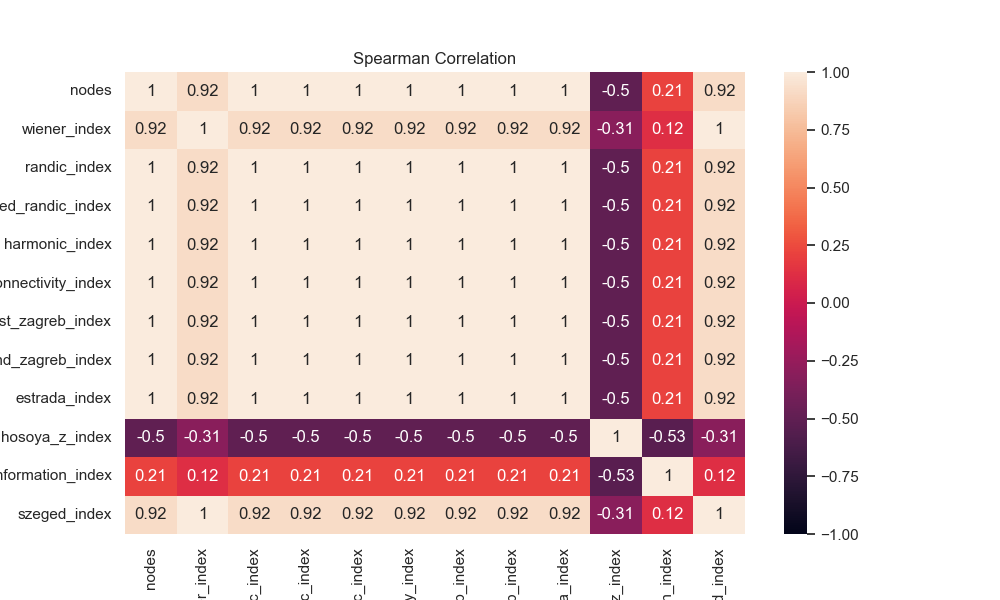
\includegraphics[width=0.7\textwidth]{images/30_results/line-correlation.png}
    \caption{Spearman-Korrelation der topologischen Indizes der Klasse \mintinline{python3}{Line}}
    \label{fig:correlation-line}
\end{figure}

Die Pfadgraphen liefern eine monoton aufsteigende Korrelation. Ebenfalls in Anhang \ref{sec:correlation-pairs} ist zu erkennen, dass die Werte der topologischen Indizes der Klasse \mintinline{python3}{Line} überaus ähnlich sind. Ihr $r$- und $p$-Wert liegt bei fast allen Indizes bei $1$.

\begin{figure}[H]
    \centering
    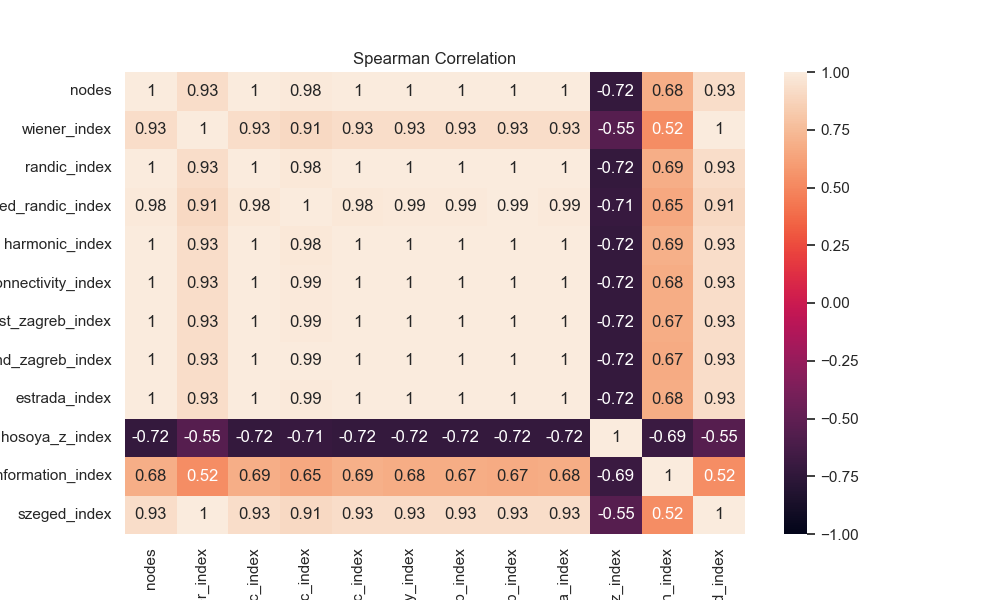
\includegraphics[width=0.7\textwidth]{images/30_results/tree-correlation.png}
    \caption{Spearman-Korrelation der topologischen Indizes der Klasse \mintinline{python3}{Tree}}
    \label{fig:correlation-tree}
\end{figure}

Die Baumgraphen liefern eine ähnliche Korrelation wie die Pfadgraphen. Auch hier ist festzustellen, dass die Werte der topologischen Indizes der Klasse \mintinline{python3}{Tree} überaus ähnlich sind. Neu zu erkennen ist jedoch der abfallende Trend beim CII und dem Hosoya-Z-Index. Dieser Trend ist auch in Anhang \ref{sec:correlation-pairs} zu sehen. Der Wiener-Index verhält sich zum Szeged-Index in etwa gleich.

\begin{figure}[H]
    \centering
    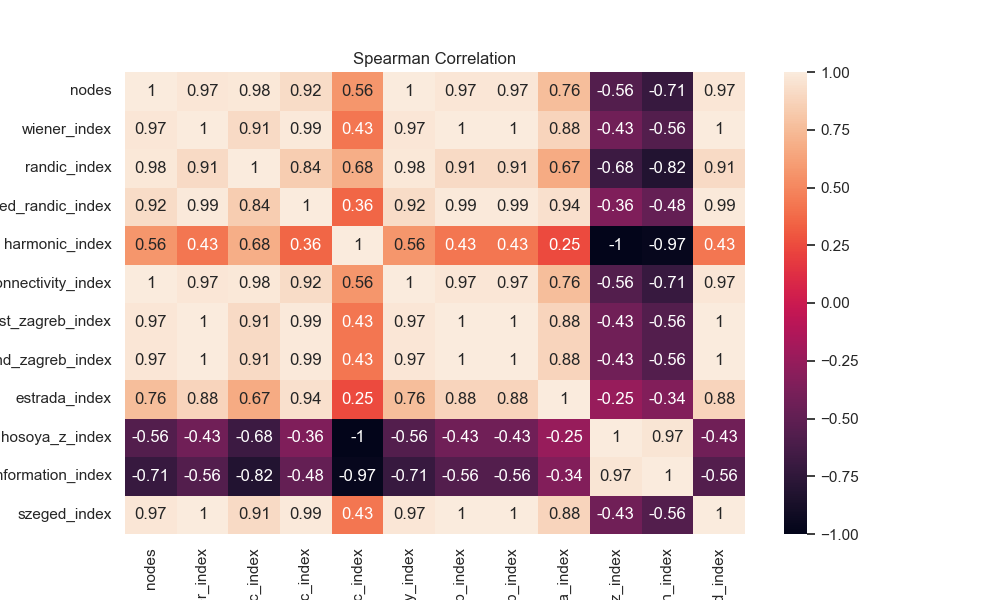
\includegraphics[width=0.7\textwidth]{images/30_results/star-correlation.png}
    \caption{Spearman-Korrelation der topologischen Indizes der Klasse \mintinline{python3}{Star}}
    \label{fig:correlation-star}
\end{figure}

Die Sterngraphenklasse liefert ein neues Bild der Heatmap. Im Durchschnitt korreliert der ABC-Index am stärksten monoton aufsteigend mit den anderen topologischen Indizes. Besonders deutlich zu sehen, ist die Korrelation aller topologischen Indizes untereinander; es gibt keine Werte, welche sich durchgehend nahe bei $0$ befinden.

\newpage

\subsection{Principal Component Analysis}

Die Principal Component Analysis (PCA) ist eine statistische Methode, mit welcher die Dimensionalität von Daten reduziert \cite{jolliffe_principal_1986} wird.
Dabei werden die Daten in eine neue Basis transformiert, welche die maximale Varianz der Daten wiedergibt.
Mathematisch wird dies durch die Eigenwerte und Eigenvektoren der Kovarianzmatrix der Daten beschrieben.

\subsubsection{Beitrag der PCA zur Usefulness}

Die PCA kann verwendet werden, um einen Datensatz aus interdependenten Variablen in einen neuen Satz von Variablen, den Hauptkomponenten, zu transformieren \cite{jolliffe_principal_1986}.
Diese Hauptkomponenten können dann analysiert werden, um Trends, Sprünge, Cluster und Ausreisser in den Daten zu beobachten.
Durch die Verwendung der PCA-Methode können wir die Nützlichkeit von topologischen Indizes für verschiedene Klassen von Graphen vergleichen.
Die PCA kann uns helfen, die wichtigsten Hauptkomponenten zu identifizieren, die zur Unterscheidung zwischen den verschiedenen Klassen von Graphen beitragen.
Auf diese Weise können wir die topologischen Indizes identifizieren, die für die verschiedenen Klassen von Graphen am nützlichsten sind.

Durch die Anwendung der PCA können die topologischen Indizes, die die grösste Varianz innerhalb der Daten erklären, identifiziert werden und somit wichtige Informationen über die Struktur der Graphen liefern \cite[p.~303]{basak_topological_1987}.

Im Jahr 1987 haben Basak et al. 90 Indizes mittels PCA auf ihre aussagekräftigste Komponente reduziert \cite{basak_topological_1987}.
Sie sind zum Resultat gekommen, dass die ersten zehn Komponenten 90 \% der Varianz der Daten beschreiben.

Durch die Anwendung der PCA auf die topologischen Indizes können die Hauptkomponenten identifiziert werden, die die meisten Informationen enthalten und somit am meisten zur Beschreibung der Struktur des Netzwerks beitragen.
Die \textbf{\textit{Usefulness}} der topologischen Indizes wird in dieser Arbeit gemessen, indem die Hauptkomponenten mit den höchsten Eigenwerten identifiziert werden.
Somit können die topologischen Indizes identifiziert werden, die die meisten Informationen enthalten und somit am meisten zur Beschreibung der Struktur des Netzwerks beitragen.
Auf diese Weise können die wichtigsten topologischen Indizes für verschiedene Klassen von Graphen identifiziert werden.

\subsubsection{PCA in scikit-learn}

Um die PCA etwas besser verstehen zu können, wird zuerst das eingegebene Datenset in einem 2D-Plot visualisiert.
Die PCA-Methode in \mintinline{python3}{scikit-learn} wurde per Randomized Singular Value Decomposition (SVD) implementiert \cite{halko_finding_2011}.
Diese Methode wird automatisch von der PCA-Methode in scikit-learn verwendet, wenn ein grosses Datenset ($> 500 \times 500$) eingegeben wird.

\subsubsection{Erklärbare Varianz}

Es wird untersucht, wie viele Principal Components (PCs) benötigt werden, um 95 \% der Varianz der Daten zu beschreiben.
Dies kann mit einem Scree-Plot dargestellt werden, der auf der x-Achse die Anzahl der PCs und auf der y-Achse die Varianz der Daten hat, welche durch die PCs beschrieben wird.

\begin{figure}[H]
    \begin{subfigure}{.5\textwidth}
        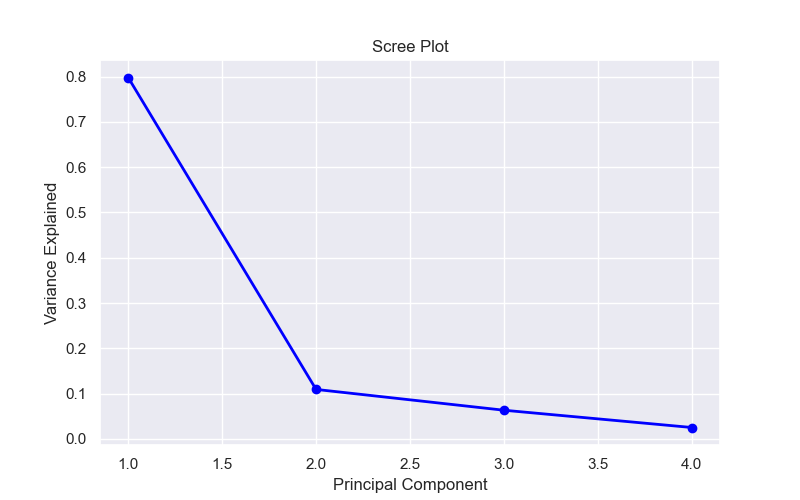
\includegraphics[width=\textwidth]{images/30_results/random-scree.png}
        \caption{Scree Plot stellt die Varianz der PC in \mintinline{python3}{Random} dar}
        \label{fig:scree-random}
    \end{subfigure}%
    \begin{subfigure}{.5\textwidth}
        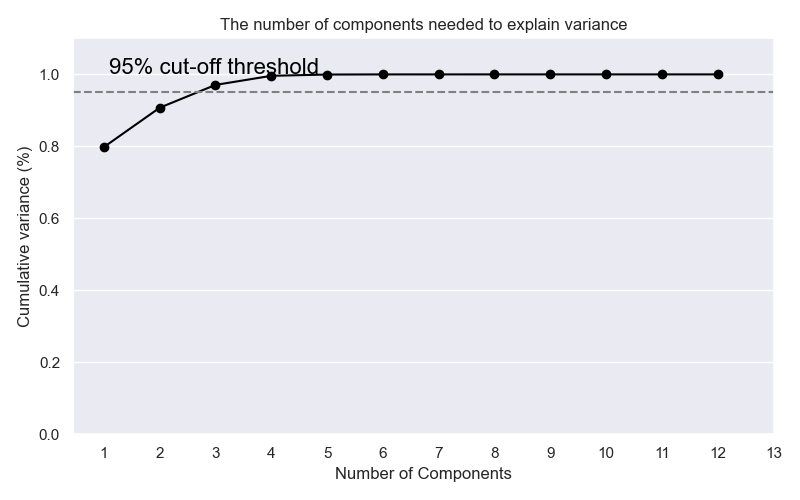
\includegraphics[width=\textwidth]{images/30_results/random-scree-cum.png}
        \caption{Scree Plot stellt die kumulative Varianz der PC in \mintinline{python3}{Random} dar}
        \label{fig:scree-cum-random}
    \end{subfigure}
\end{figure}

\medskip

\begin{figure}
    \ContinuedFloat
    \begin{subfigure}{.5\textwidth}
        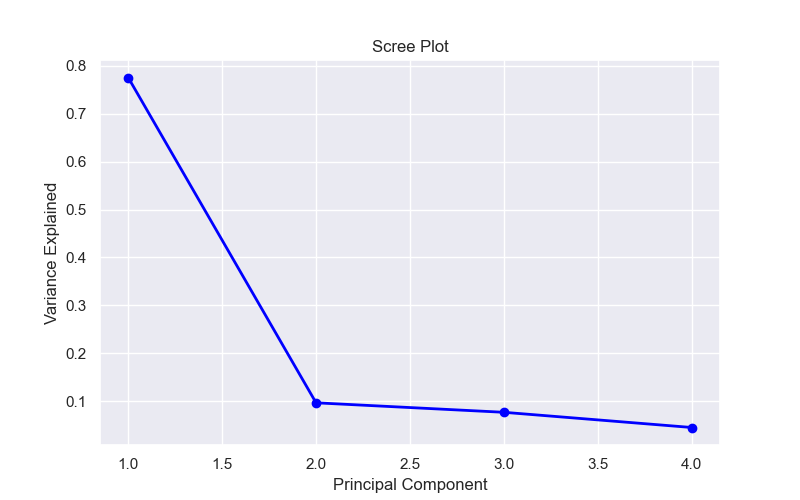
\includegraphics[width=\textwidth]{images/30_results/smallworld-scree.png}
        \caption{Scree Plot stellt die Varianz der PC in \mintinline{python3}{Small-World} dar}
        \label{fig:scree-smallworld}
    \end{subfigure}%
    \begin{subfigure}{.5\textwidth}
        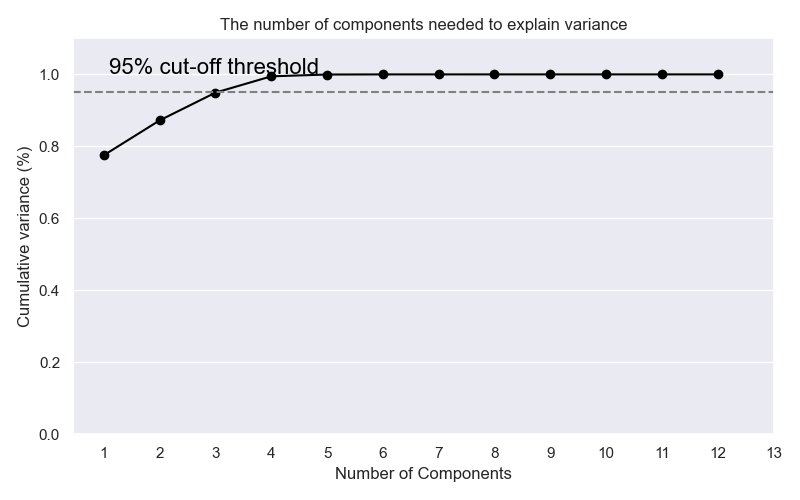
\includegraphics[width=\textwidth]{images/30_results/smallworld-scree-cum.png}
        \caption{Scree Plot stellt die kumulative Varianz der PC in \mintinline{python3}{Small-World} dar}
        \label{fig:scree-cum-smallworld}
    \end{subfigure}

    \begin{subfigure}{.5\textwidth}
        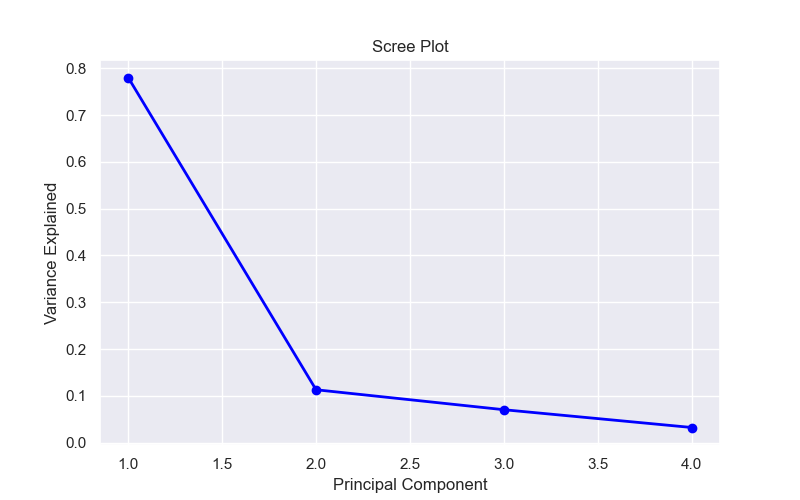
\includegraphics[width=\textwidth]{images/30_results/scalefree-scree.png}
        \caption{Scree Plot stellt die Varianz der PC in \mintinline{python3}{Scale-free} dar}
        \label{fig:scree-scalefree}
    \end{subfigure}%
    \begin{subfigure}{.5\textwidth}
        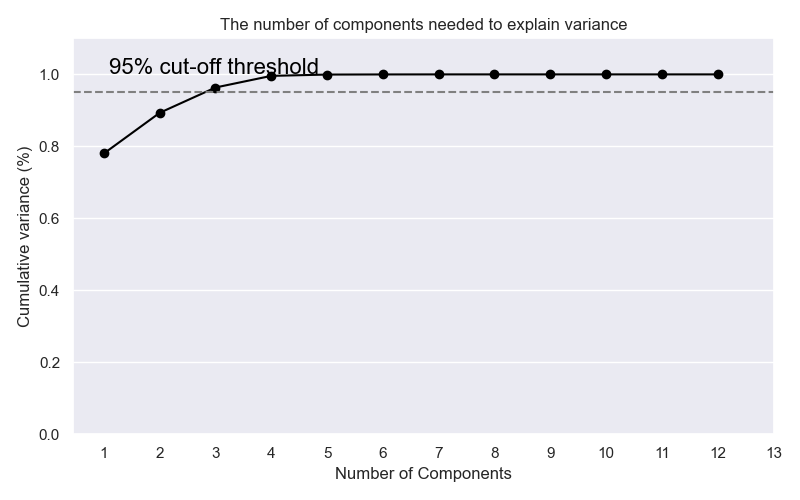
\includegraphics[width=\textwidth]{images/30_results/scalefree-scree-cum.png}
        \caption{Scree Plot stellt die kumulative Varianz der PC in \mintinline{python3}{Scale-free} dar}
        \label{fig:scree-cum-scalefree}
    \end{subfigure}
    \ContinuedFloat
    \begin{subfigure}{.5\textwidth}
        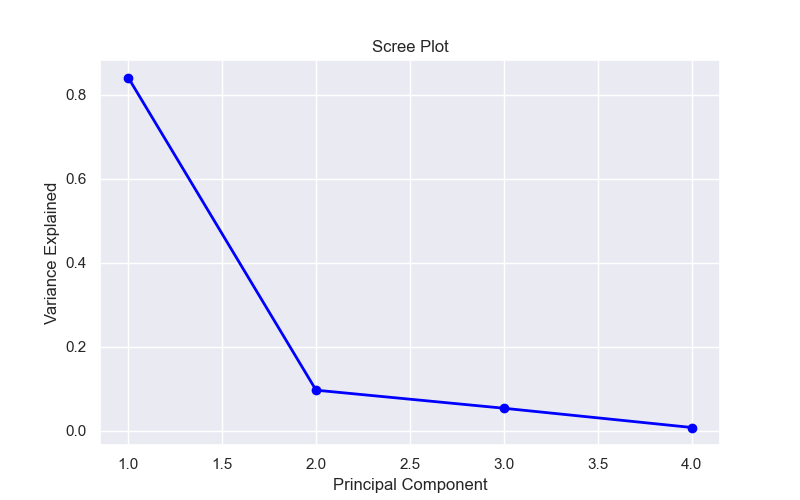
\includegraphics[width=\textwidth]{images/30_results/complete-scree.png}
        \caption{Scree Plot stellt die Varianz der PC in \mintinline{python3}{Complete} dar}
        \label{fig:scree-complete}
    \end{subfigure}%
    \begin{subfigure}{.5\textwidth}
        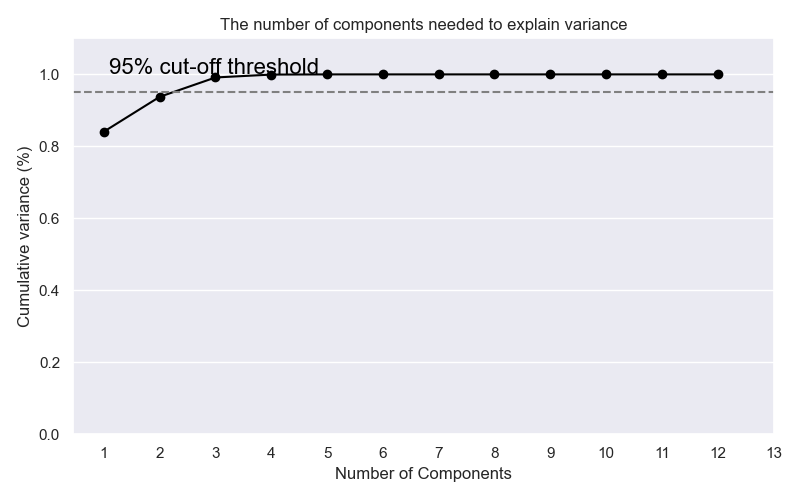
\includegraphics[width=\textwidth]{images/30_results/complete-scree-cum.png}
        \caption{Scree Plot stellt die kumulative Varianz der PC in \mintinline{python3}{Complete} dar}
        \label{fig:scree-cum-complete}
    \end{subfigure}
\end{figure}

\medskip

\begin{figure}
    \ContinuedFloat
    \begin{subfigure}{.5\textwidth}
        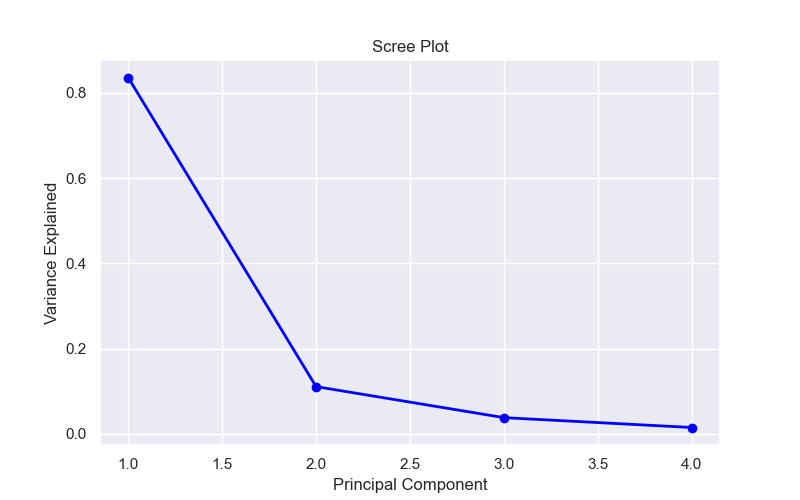
\includegraphics[width=\textwidth]{images/30_results/line-scree.png}
        \caption{Scree Plot stellt die Varianz der PC in \mintinline{python3}{Line} dar}
        \label{fig:scree-line}
    \end{subfigure}%
    \begin{subfigure}{.5\textwidth}
        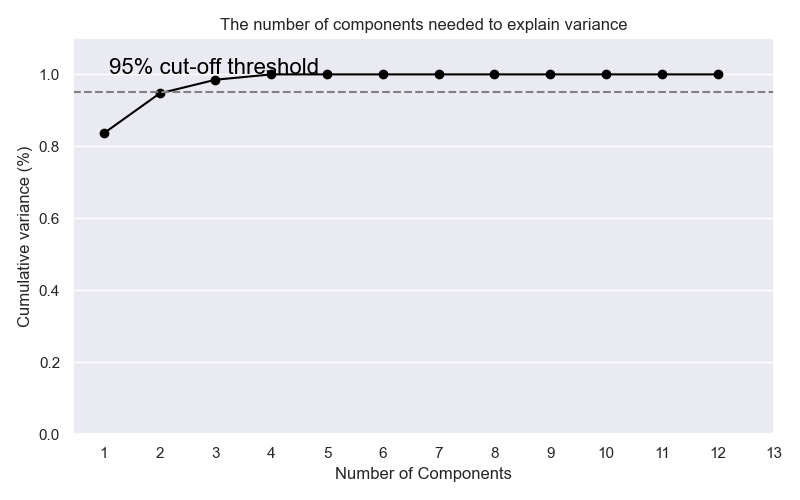
\includegraphics[width=\textwidth]{images/30_results/line-scree-cum.png}
        \caption{Scree Plot stellt die kumulative Varianz der PC in \mintinline{python3}{Line} dar}
        \label{fig:scree-cum-line}
    \end{subfigure}

    \begin{subfigure}{.5\textwidth}
        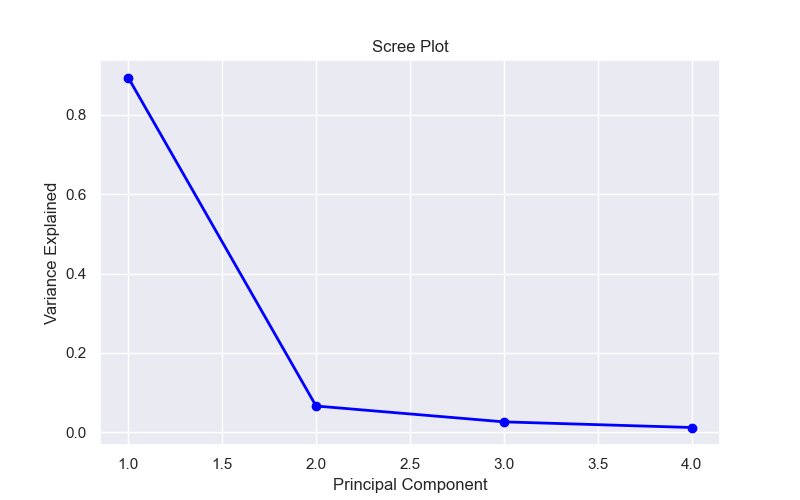
\includegraphics[width=\textwidth]{images/30_results/tree-scree.png}
        \caption{Scree Plot stellt die Varianz der PC in \mintinline{python3}{Tree} dar}
        \label{fig:scree-tree}
    \end{subfigure}%
    \begin{subfigure}{.5\textwidth}
        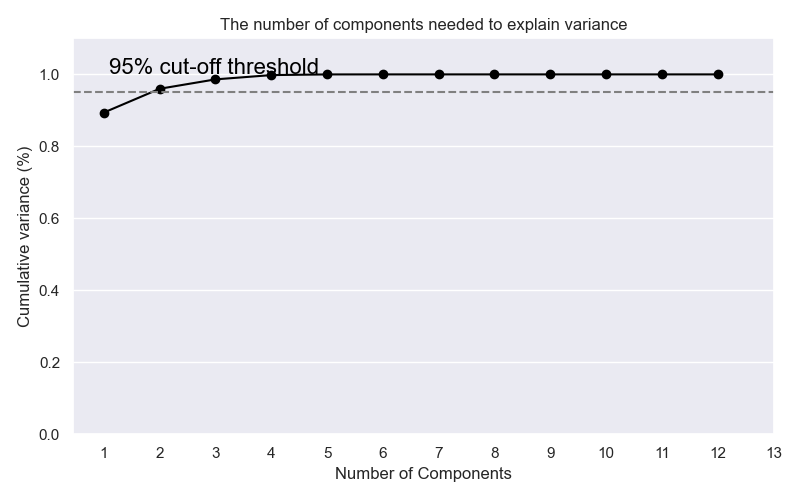
\includegraphics[width=\textwidth]{images/30_results/tree-scree-cum.png}
        \caption{Scree Plot stellt die kumulative Varianz der PC in \mintinline{python3}{Tree} dar}
        \label{fig:scree-cum-tree}
    \end{subfigure}

    \begin{subfigure}{.5\textwidth}
        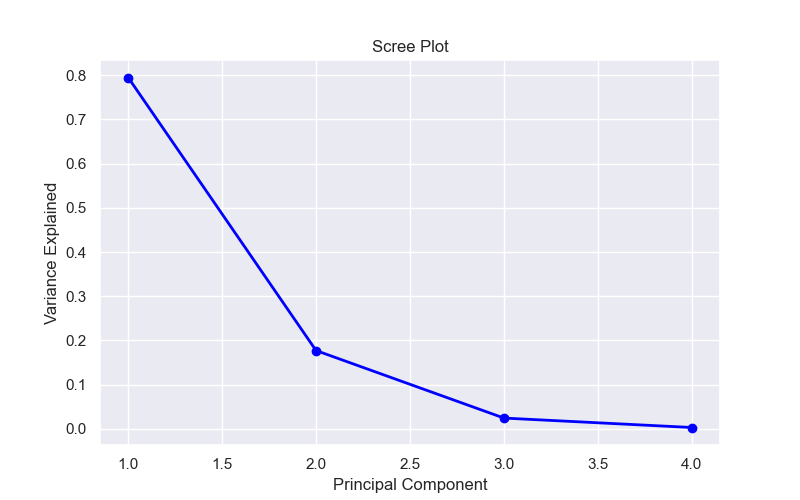
\includegraphics[width=\textwidth]{images/30_results/star-scree.png}
        \caption{Scree Plot stellt die Varianz der PC in \mintinline{python3}{Star} dar}
        \label{fig:star-line}
    \end{subfigure}%
    \begin{subfigure}{.5\textwidth}
        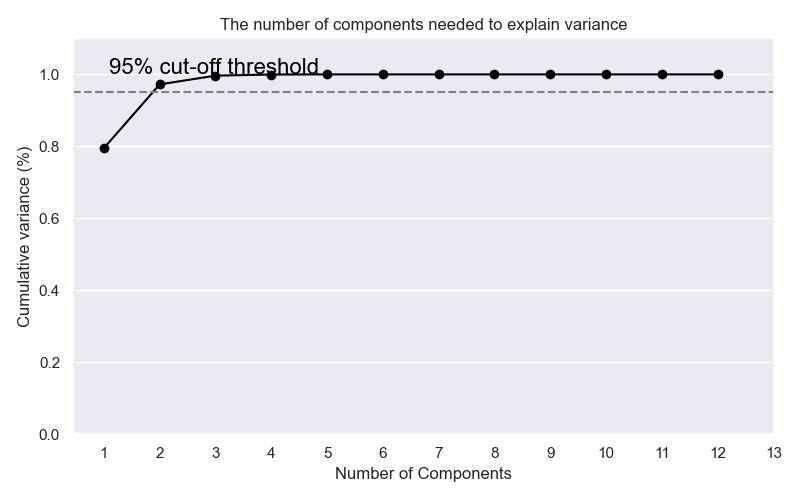
\includegraphics[width=\textwidth]{images/30_results/star-scree-cum.png}
        \caption{Scree Plot stellt die kumulative Varianz der PC in \mintinline{python3}{Star} dar}
        \label{fig:scree-cum-star}
    \end{subfigure}
\end{figure}

Auf allen Abbildung von \ref{fig:scree-random} bis \ref{fig:scree-cum-star} ist zu erkennen, dass die Varianz der ersten Komponente überaus hoch ist. Die erklärbare Varianz von 95 \% wird in allen Klassen mit maximal vier Komponenten erreicht. In den meisten Klassen reichen zwei Komponenten aus.
Bei den Baum- und Sterngraphen genügt sogar eine Komponente, um 95 \% der Varianz zu erklären.

\newpage

\paragraph{PCA-Loadings}

Als Nächstes folgen die Loadings der PCA-Methode. Die Eigenvektoren der PCs geben die Richtung der Komponenten an, während die Eigenwerte die Varianz der Komponenten beschreiben.
Die Loadings, auch $Q$-Matrix genannt, sind die Gewichte der einzelnen Variablen, welche die Komponenten beschreiben \cite[p.~434]{abdi_principal_2010}.
Im Wesentlichen zeigen die Loadings, wie stark jede Variable mit jeder der Hauptkomponenten korreliert. Hohe positive Loadings zeigen an, dass eine Variable stark mit einer bestimmten Hauptkomponente korreliert, während hohe negative Loadings anzeigen, dass die Variable eine starke negative Korrelation mit der Hauptkomponente aufweist.
Die Loadings können verwendet werden, um zu verstehen, welche Variablen in den Daten am meisten zur Variabilität beitragen und wie die Variablen miteinander zusammenhängen \cite[p.~438]{abdi_principal_2010}.

Sie werden nachfolgend in einem 2D-Plot visualisiert, wobei die x-Achse die erste Komponente und die y-Achse die zweite Komponente wiedergibt, und Folgendermassen berechnet:

\begin{equation}
    \label{eq:loadings}
    \text{Loadings} = \text{Eigenvektoren} \cdot \sqrt{\text{Eigenwerte}}
\end{equation}

\begin{figure}[H]
    \centering
    \begin{subfigure}{.5\textwidth}
        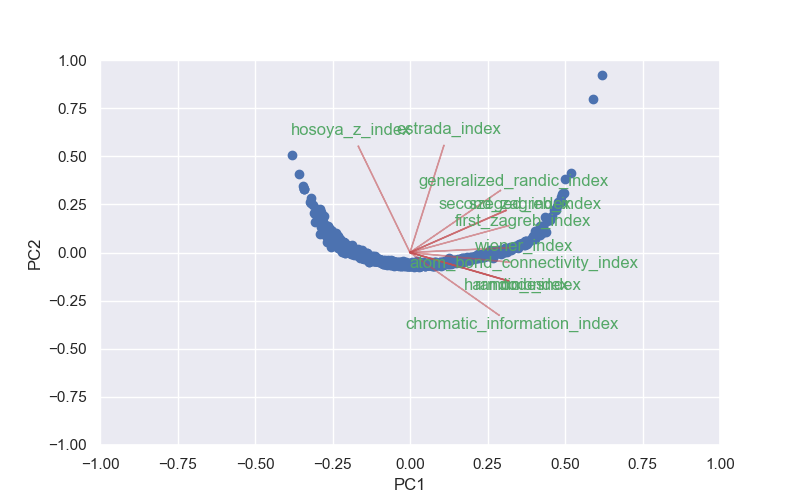
\includegraphics[width=\textwidth]{images/30_results/random-pca-loadings.png}
        \caption{Loading Plots der 2-PCA Methode der Klasse \mintinline{python3}{Random}}
        \label{fig:pca-loading-random}
    \end{subfigure}%
    \begin{subfigure}{.5\textwidth}
        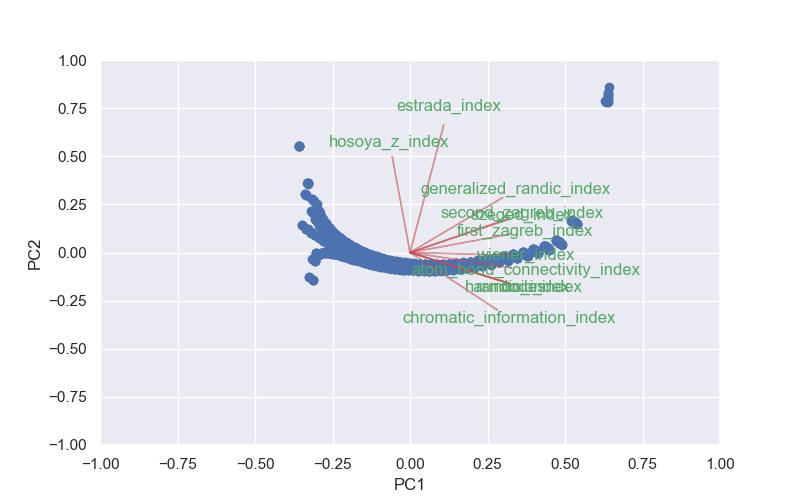
\includegraphics[width=\textwidth]{images/30_results/smallworld-pca-loadings.png}
        \caption{Loading Plots der 2-PCA Methode der Klasse \mintinline{python3}{Small-World}}
        \label{fig:pca-loading-smallworld}
    \end{subfigure}

    \begin{subfigure}{.5\textwidth}
        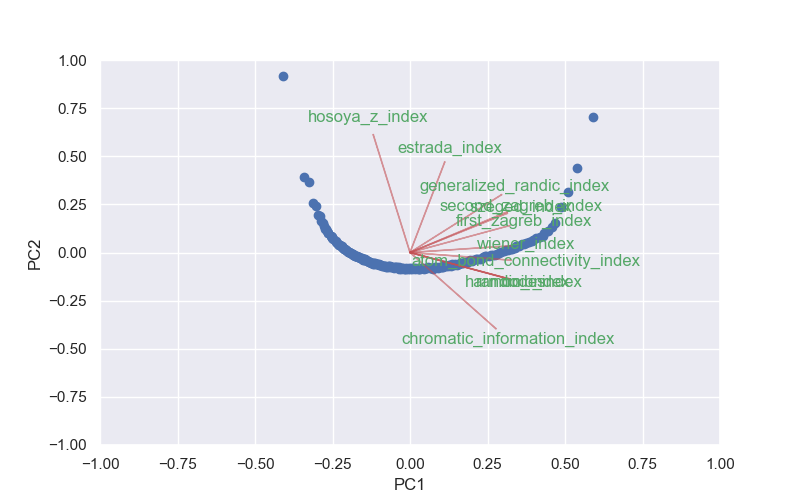
\includegraphics[width=\textwidth]{images/30_results/scalefree-pca-loadings.png}
        \caption{Loading Plots der 2-PCA Methode der Klasse \mintinline{python3}{Scale-free}}
        \label{fig:pca-loading-scalefree}
    \end{subfigure}%
    \begin{subfigure}{.5\textwidth}
        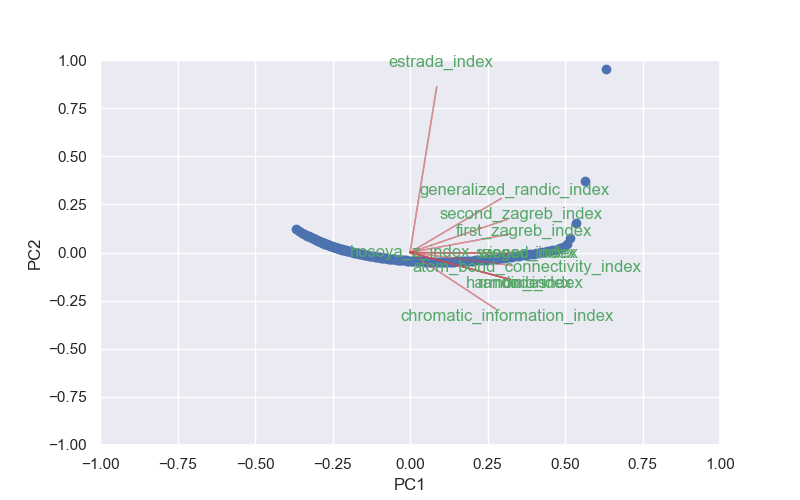
\includegraphics[width=\textwidth]{images/30_results/complete-pca-loadings.png}
        \caption{Loading Plots der 2-PCA Methode der Klasse \mintinline{python3}{Complete}}
        \label{fig:pca-loading-complete}
    \end{subfigure}
\end{figure}


\begin{figure}[H]
    \ContinuedFloat
    \centering
    \begin{subfigure}{.5\textwidth}
        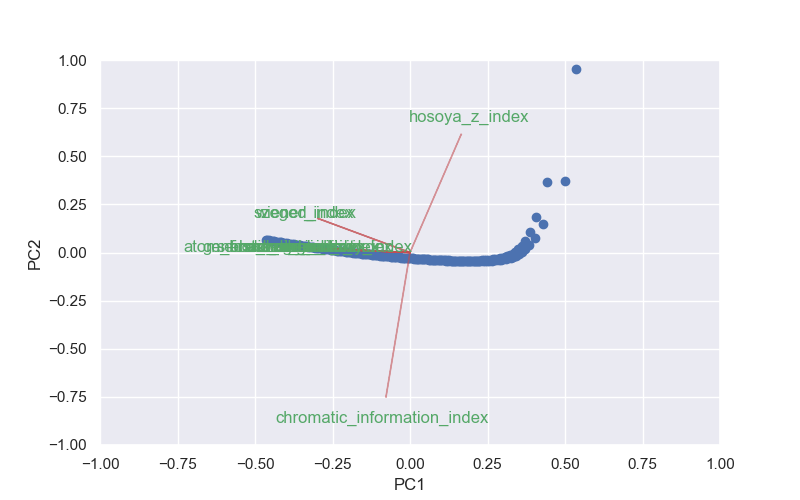
\includegraphics[width=\textwidth]{images/30_results/line-pca-loadings.png}
        \caption{Loading Plots der 2-PCA Methode der Klasse \mintinline{python3}{Line}}
        \label{fig:pca-loading-line}
    \end{subfigure}%
    \begin{subfigure}{.5\textwidth}
        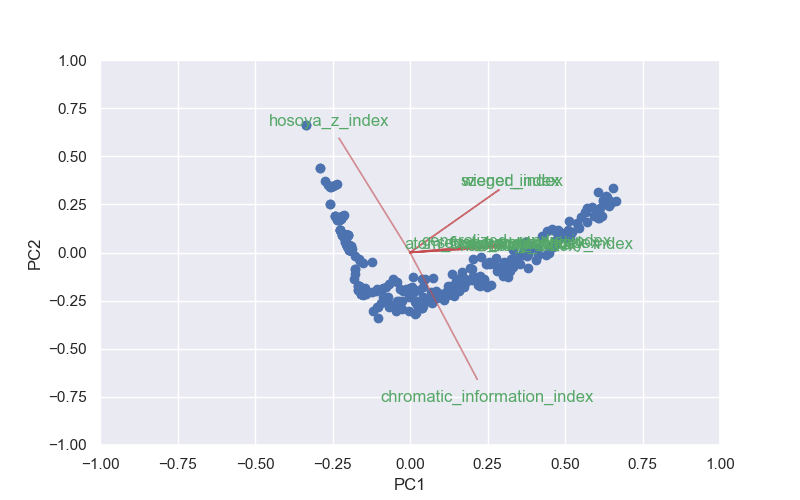
\includegraphics[width=\textwidth]{images/30_results/tree-pca-loadings.png}
        \caption{Loading Plots der 2-PCA Methode der Klasse \mintinline{python3}{Tree}}
        \label{fig:pca-loading-tree}
    \end{subfigure}
\end{figure}

\begin{figure}[H]
    \ContinuedFloat
    \centering
    \begin{subfigure}{0.8\textwidth}
        \centering
        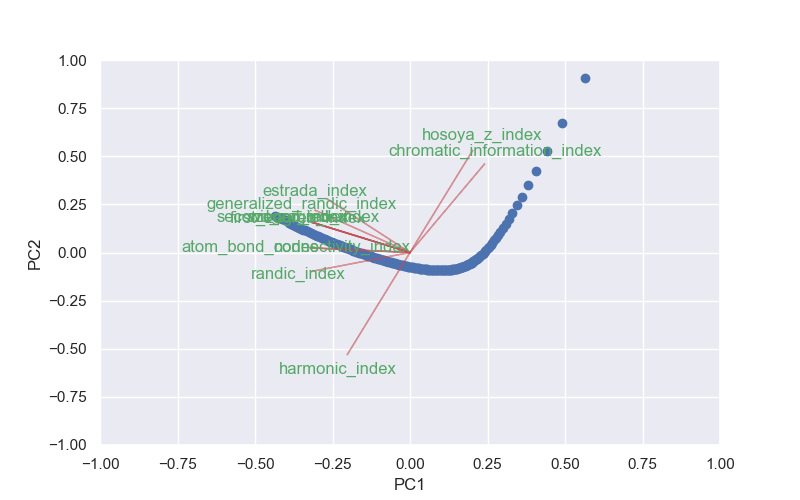
\includegraphics[width=0.8\textwidth]{images/30_results/star-pca-loadings.png}
        \caption{Loading Plots der 2-PCA Methode der Klasse \mintinline{python3}{Star}}
        \label{fig:pca-loading-star}
    \end{subfigure}%
\end{figure}

Die Loadings der PCs zeigen, wie die topologischen Indizes zur Komponente beitragen.
Ähnlich wie bei der Spearman-Korrelation bedeuten positive Loadings, dass der Index eine positive Korrelation zur Komponente hat; negative Loadings entsprechen einer negativen Korrelation. Je höher der Wert ist, desto stärker ist die Korrelation \cite{bartl_statistik_2017}. Für uns bedeutet das, dass die Indizes mit hohen positiven Loadings die Komponente stark beeinflussen.

Die Eigenwerte $ \lambda $ der Komponenten speichern die Varianz der Komponenten und die Eigenvektoren $ \vec{v} $ die Richtung der Komponenten. Werden nun $ \lambda $ auf $ \vec{v} $ übertragen, so erhält man die PC-Loadings. Diese Loadings enthalten, da sie Varianz als auch Richtung enthalten, die Kovarianz zwischen den ursprünglichen Werten und den PCs \cite[p.~438]{abdi_principal_2010}.

\newpage

\subsubsection{Einfluss der Komponenten}

Zum Schluss der Korrelationsanalyse werden die einzelnen Komponenten der PCA-Methode der jeweiligen Klassen identifiziert.
Mittels der den Scree-Plots lässt sich feststellen, dass bei den überwiegenden Klassen die ersten zwei Komponenten die meisten Informationen über die Daten enthalten.
Deshalb werden die einzelnen Komponenten der Klasse \mintinline{python3}{Random} bei den Hauptkomponenten zur Analyse ausgegeben.

\begin{table}[H]
    \caption{PCA-Komponenten der Erdős-Rényi-Klasse und der Einfluss der Indizes auf die Komponenten}
    \begin{adjustbox}{minipage=\textwidth, center}
        \tiny
        \begin{tabularx}{\textwidth}{l c c c c c c c c c c c}
            \hline
                          & wiener         & randic & g. randic & harmonic & abc    & 1st zagreb & 2nd zagreb & estrada        & z              & cii    & szeged \\ \hline
            \textbf{PC-1} & \textbf{0.338} & 0.331  & 0.310     & 0.331    & 0.337  & 0.334      & 0.327      & 0.119          & -0.172         & 0.297  & 0.327  \\
            \textbf{PC-2} & 0.007          & -0.165 & 0.303     & -0.165   & -0.068 & 0.121      & 0.200      & 0.554          & \textbf{0.575} & -0.342 & 0.198  \\
            \textbf{PC-3} & -0.113         & -0.019 & -0.075    & -0.019   & -0.077 & -0.131     & -0.123     & \textbf{0.784} & -0.544         & 0.128  & -0.127 \\
            \textbf{PC-4} & 0.057          & 0.258  & -0.379    & 0.258    & 0.166  & -0.103     & -0.230     & 0.239          & \textbf{0.576} & 0.431  & -0.235 \\ \hline
        \end{tabularx}
    \end{adjustbox}
    \label{table:pca_components}
\end{table}

In Tabelle \ref{table:pca_components} ist der Einfluss der Variablen (hier topologische Indizes) auf die Komponenten der Klasse \mintinline{python3}{Random} dargestellt.
Es ist ersichtlich, dass der Wiener-Index den stärksten Einfluss auf die erste Hauptkomponente hat, der Hosoya-Z-Index auf die zweite und vierte und der Estrada-Index auf die dritte Komponente.
Die abschliessende Liste aller Einflüsse der topologischen Indizes auf die Komponenten der Klassen ist in Anhang \ref{sec:ti-pca} ersichtlich.

Die Tabelle \ref{table:pca_components} zeigt die Loadings der Hauptkomponenten für die Klasse \mintinline{python3}{Random}. Anhand dieser Loadings kann die Einflüsse der verschiedenen topologischen Indizes auf die Hauptkomponenten dieser Klasse bestimmt werden. Der Index mit dem höchsten Einfluss ist schliesslich der nützlichste Index für diese Klasse. Die Herleitung dieser Aussage wird anhand der Definition \ref{thm:useful_index} und der darauffolgenden Beschreibung gezeigt.

\subsubsection{Meine Definition des \textit{nützlichen} topologischen Index}

Somit ist es nun möglich, die Hauptdefinition und Beantwortung der Forschungsfrage 1 und 2 zu finden.

\begin{theorem}[\textbf{nützlicher} topologischer Index $\Phi$]
    \label{thm:useful_index}%
    Je höher der Einfluss eines topologischen Index auf die Hauptkomponenten seiner Klasse ist, desto höher ist dessen \textbf{Usefulness}.
\end{theorem}

Für dieses Theorem muss definiert werden, was mit \textit{Einfluss} gemeint ist.
Der Einfluss eines topologischen Index auf die PCs einer Klasse lässt sich anhand der Loadings der Komponenten bestimmen.
Sind die Loadings eines Index hoch positiv, so korreliert der Index positiv mit der Komponente.
Die Loading-Werte der Komponenten werden in Tabelle \ref{table:pca_components} für die Klasse \mintinline{python3}{Random} dargestellt.

Die Formel zur Berechnung der Usefulness eines topologischen Index auf die Hauptkomponenten seiner Klasse kann wie folgt definiert werden:

\begin{equation}
    \label{eq:index_usefulness}
    \Phi_{i} = \sum_{j=1}^{m} |w_{ij}| \cdot \sigma^2_j
\end{equation}

Wobei $i$ dem Index des topologischen Indizes in dem Datenset entspricht, $m$ der Anzahl der Hauptkomponenten und $j$ die $j$-te Hauptkomponente. $w_{ij}$ ist das Loading des topologischen Indizes $i$ auf der $j$-ten Hauptkomponente.
Die Werte der Loadings $w_{ij}$ werden mit der $j$-ten Hauptkomponente aufsummiert und diese danach  mit der erklärbaren Varianz $\sigma^2$ der $j$-ten Hauptkomponente multipliziert.

Die erklärbare Varianz $\sigma^2$ der Hauptkomponenten für die Klasse \mintinline{python3}{Random} lautet:

% Mint Code-Listing
\begin{listing}[H]
    \begin{minted}
    [frame=lines,framesep=2mm,baselinestretch=1.2,bgcolor=LightGray,fontsize=\footnotesize,linenos]
    {text}    
------------ PCA random 4 explained variance ratio ------------
        explained variance ratio
  PC-1                     0.784
  PC-2                     0.116
  PC-3                     0.069
  PC-4                     0.026
    \end{minted}
    \caption{Erklärbare Varianz der Hauptkomponenten der Klasse \mintinline{python3}{Random}}
\end{listing}

Nach Anwendung der Formel \ref{eq:index_usefulness} werden die Daten mit der MinMax-Normalisierung $ \bar{\Phi}_{i} = \frac{(\Phi_i - \min_x)}{(\max_x - \min_x)} $ normalisiert, wobei $x$ das berechnete Datenset für alle $ \Phi $ der Graphenklasse $ \mathcal{N} $ ist.
Für den Wiener-Index und die Random-Klasse sind die Loadings in der ersten Komponente in Tabelle \ref{table:pca_components} gegeben. Wir sehen, dass das Loading des Wiener-Index in der ersten Komponente $0.338$ beträgt.

Um die Formel \ref{eq:index_usefulness} zu testen, wird der Einfluss des Wiener-Index und Randić-Index auf die Random-Graphenklasse berechnet.

\begin{equation}
    \label{eq:test_index_usefulness}
    \begin{aligned}
        \Phi_{wiener}       & = |0.338| \cdot 0.784 + |0.007| \cdot 0.116 + |-0.113| \cdot 0.069 + |0.057| \cdot 0.026  \\
                            & = 0.275100                                                                                \\
        \bar{\Phi}_{wiener} & = 0.747183                                                                                \\
        \Phi_{randic}       & = |0.331| \cdot 0.784 + |-0.165| \cdot 0.116 + |-0.019| \cdot 0.069 + |0.258| \cdot 0.026 \\
                            & = 0.286618                                                                                \\
        \bar{\Phi}_{randic} & = 0.899278
    \end{aligned}
\end{equation}

Die Normalisierung der Usefulness der topologischen Indizes auf die Hauptkomponenten der Klasse \mintinline{python3}{Random} ergibt folgende Werte:

% Mint Code-Listing
\begin{listing}[H]
    \begin{minted}
    [frame=lines,framesep=2mm,baselinestretch=1.2,bgcolor=LightGray,fontsize=\footnotesize,linenos]
    {text}    
------------ PCA random combined usefulness score ------------
index                      usefulness score
wiener                     0.747183
randic                     0.899278
generalized_randic         0.985581
harmonic                   0.899467
abc                        0.833882
1st zagreb                 0.915968
2nd zagreb                 0.998606
estrada                    0.000000
z                          0.476098
cii                        0.985445
szeged                     1.000000
    \end{minted}
    \caption{Usefulness-Score aller topologischen Indizes für die Graphenklasse \mintinline{python3}{Random}}
\end{listing}

Das Theorem \ref{thm:useful_index} besagt nun, dass der topologische Index \textit{useful} ist, wenn sein Einfluss auf die Hauptkomponenten seiner Klasse am höchsten ist. Der Einfluss lässt sich anhand der Loadings der Komponenten bestimmen, wie in der Formel \ref{eq:index_usefulness} beschrieben.

\subsubsection{Scoring aller Klassen und Indizes}

Nachdem der Einfluss der Indizes auf die Varianz der Hauptkomponenten innerhalb einer Klasse von Graphen untersucht ist, wird nun eine Reihenfolge der bedeutendsten Indizes für jede Klasse präsentiert.
Dabei liegt der Fokus auf den ersten vier Hauptkomponenten, da diese in allen Fällen über 95 \% der Daten erklärt werden können.
Im nachfolgenden Listing sind die 3 wichtigsten Indizes für jede Klasse aufgelistet. Alle Indizes, sowie alle erklärbare Varianzen der Hauptkomponenten sind unter Anhang \ref{sec:all_pca} zu finden.

% Mint Code-Listing
\begin{listing}[H]
    \begin{minted}
        [frame=lines,framesep=2mm,baselinestretch=1.2,bgcolor=LightGray,fontsize=\footnotesize,linenos]
        {text}    
------------ PCA random combined usefulness score ------------
                           influence score
szeged                     1.000000
2nd zagreb                 0.998606
generalized_randic         0.985581

------------ PCA smallworld combined usefulness score ------------
                           influence score
generalized_randic         1.000000
harmonic                   0.985451
randic                     0.985409

------------ PCA scalefree combined usefulness score ------------
                   influence score
2nd zagreb         1.000000
szeged             0.999622
cii                0.989833

------------ PCA complete combined usefulness score ------------
                           influence score
generalized_randic         1.000000
2nd zagreb                 0.990307
randic                     0.987024

------------ PCA line combined usefulness score ------------
                           influence score
szeged                     1.000000
wiener                     1.000000
generalized_randic         0.848312

------------ PCA tree combined usefulness score ------------
                   influence score
szeged             1.000000
wiener             0.999889
2nd zagreb         0.692432

------------ PCA star combined usefulness score ------------
                           influence score
generalized_randic         1.000000
estrada                    0.778188
szeged                     0.719018
    \end{minted}
    \caption{Ausgabe der Scores der Indizes mit der höchsten Usefulness innerhalb der Graphenklassen. Bei allen Random-Graphen besitzt der Szeged-Index den höchsten Einfluss über alle Hauptkomponenten. Bei den Pfad-Graphen haben der Szeged- und Wiener-Index denselben Usefulness-Score.}
\end{listing}

Aus den Ergebnissen der Usefulness-Scores wird ersichtlich, dass bei der Graphenklasse \mintinline{python3}{Star} der Generalized-Randić-Index den höchsten Abstand zu den anderen Indizes hat. Hier eignet sich der Index besonders zur Verwendung und ist damit nützlicher als die anderen Masse. Der Generalized-Randić-Index hat den höchsten Einfluss auf die vier Hauptkomponenten der Klasse \mintinline{python3}{Star}.
Bei den anderen Graphenklassen sind die Scores der ersten drei Indizes sehr ähnlich.

Jedoch auch die Bäume besitzen nach den ersten beiden Indizes, dem Szeged- und Wiener-Index einen Abstand zu den anderen Indizes.

Den niedrigsten Usefulness-Score für die definierten Graphenklassen haben der CII- (Bäume, Pfad), Hosoya-Z (Small-World, Vollständig, Stern) und Estrada-Index (Scale-free, Random).

\section{Klassifizierung der Graphen} \label{sec:classification}

Nach der Korrelation der Graphen folgt deren Klassifizierung.
Es wird dazu ein Modell entwickelt, welches die Graphen in verschiedene Kategorien klassifiziert.
Die Theorie zur Klassifizierung der Graphen wurde in Kapitel \ref{sec:classification_theory} erläutert. Nun folgen die Anwendung der hergeleiteten Theorie und deren Resultate.

\subsection{Beschreibung des Modells}

Das Modell lehnt sich an das Graph-Convolutional-network (GCN)-Modell von \cite{kipf_semi-supervised_2017} an.
Es besteht aus drei \mintinline{python3}{GCNConv}-Schichten, einer \mintinline{python3}{Pooling}- und einer \mintinline{python3}{Linear}-Schicht.

\begin{figure}[H]
    \centering
    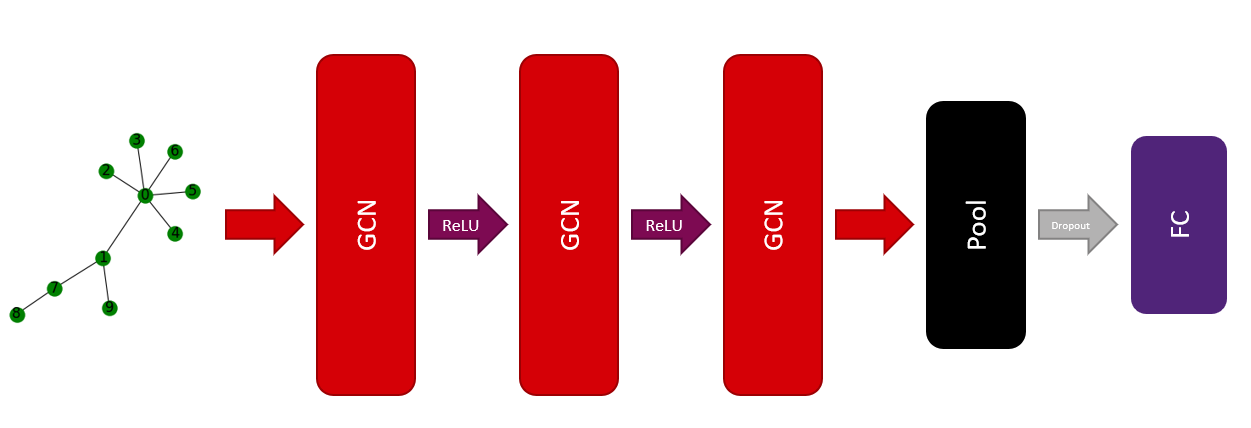
\includegraphics[width=0.8\textwidth]{images/30_results/nn_architecture.png}
    \caption{Modell für die Graphenklassifizierung (Quelle: Eigene Darstellung)}
    \label{fig:model}
\end{figure}

Die Drei \mintinline{python3}{GCNConv}-Schichten sind als Node-Embedding-Schichten zu verstehen.
\begin{equation}
    X' = \hat{D}^{-1/2} \hat{A} \hat{D}^{-1/2} X \Theta
\end{equation}
$\hat{A} = A + I$ ist die Adjazenzmatrix des Graphen mit eingefügten Schleifen $ \hat{D}_{ii} = \sum_{j=0}{\hat{A}_{ij}} $ und der diagonalen Gradmatrix.
Danach folgt eine $ReadOut$-Schicht. Diese existiert, um die einzelnen Node-Embeddings in ein Graph-Embedding zu überführen.
\begin{equation}
    X_{\mathcal{G}} = \frac{1}{\mathcal{V}} \sum_{v \in {\mathcal{V}}}{x_v^{(L)}}
\end{equation}
Es wird mit einer $Dropout$-Schicht \cite{srivastava_dropout_2014} gearbeitet, um Overfitting zu verhindern.
Zum Schluss folgt der Classifier, welcher die Graphen in die Kategorien klassifiziert.

Als Aktivierungsfunktion wird $ ReLU(x) = \max(x, 0) $ verwendet. Die Optimierung der Lernrate erfolgt adaptiv mit $Adam$ \cite{kingma_adam_2017} und dem Parameter $ 0.01 $.
Für die Multi-Class-Klassifizierung wird die Loss-Funktion Crossentropy verwendet.

\subsection{Training des Modells}

Zur Reproduktion und Evaluation folgt die Deklaration der genutzten Hardware und der Daten, die beim Training verwendet wurden.

\begin{table}[H]
    \begin{adjustbox}{minipage=\textwidth, center}
        \scriptsize
        \begin{tabularx}{\textwidth}{|l|X|}
            \hline
            \textbf{Komponente} & \textbf{Beschreibung}                  \\
            \hline
            Prozessor           & AMD Ryzen 9 3900X (24 Cores)           \\
            Arbeitsspeicher     & 64 GB DDR4 3600 MHz                    \\
            Grafikkarte         & NVIDIA GeForce RTX 2080 Ti (CUDA 11.6) \\
            Betriebssystem      & Windows 11 Pro                         \\
            \hline
        \end{tabularx}
    \end{adjustbox}
    \caption{\label{tab:tech-spec}Technische Komponenten für das Training}
\end{table}

Das Datenset besteht aus 3200 Graphen mit verschiedener Anzahl Knoten, siehe Tabelle \ref{data-table}. 
Die Knoten haben jeweils drei Features (Degree, Density und Betweenness), welche für das Node-Embedding verwendet werden.
Die Multi-Class-Klassifizierung hat sieben Klassen (siehe Tabelle \ref{data-table}). Die Graphen werden in 80 \% Trainings- und 20 \% Testdaten aufgeteilt, was eine Trainingsmenge von 2560 Graphen und eine Testmenge von 640 Graphen ergibt.
Die Test- und Trainingsdaten werden in Batches à 64 Graphen unterteilt.

Nach 62 Minuten und 32 Sekunden Training in 170 Epochen, hat das Modell eine Genauigkeit von 93 \% erreicht. 

\begin{listing}[H]
    \begin{minted}[frame=lines,framesep=2mm,baselinestretch=1.2,bgcolor=LightGray,fontsize=\footnotesize,linenos]{text}
        Output exceeds the size limit. Open the full output data in a text editor
        Epoch: 001, Train Acc: 0.1667, Test Acc: 0.1778
        Epoch: 002, Train Acc: 0.2417, Test Acc: 0.2259
        Epoch: 003, Train Acc: 0.3933, Test Acc: 0.3907
        Epoch: 004, Train Acc: 0.5200, Test Acc: 0.5204
        ...
        Epoch: 167, Train Acc: 0.9816, Test Acc: 0.9750
        Epoch: 168, Train Acc: 0.8828, Test Acc: 0.8906
        Epoch: 169, Train Acc: 0.9238, Test Acc: 0.9313
        Epoch: 170, Train Acc: 0.9258, Test Acc: 0.9344
    \end{minted}
    \caption{Verbesserung der Genauigkeit des Modells während des Trainings}
\end{listing}

Im nächsten Bild ist die Genauigkeit über die 170 Epochen dargestellt.
Es ist ersichtlich, dass die Genauigkeit vorwiegend in den ersten 25 Epochen stark zunimmt.
Ab der 100. Epoche gibt es nochmals einen kleinen Anstieg von 0.5 \%.

Auf Abbildung \ref{fig:wandb_dashboard} im Anhang \ref{sec:wandb_dashboard} eine Dashboard-Ansicht von Weights and Biases \cite{wandb}, welches die Genauigkeit und die Loss-Funktion über die Epochen darstellt.
Durch das Hochladen der Trainings- und Testdaten können auch die falschen Klassifizierungen analysiert werden.

\begin{figure}[H]
    \centering
    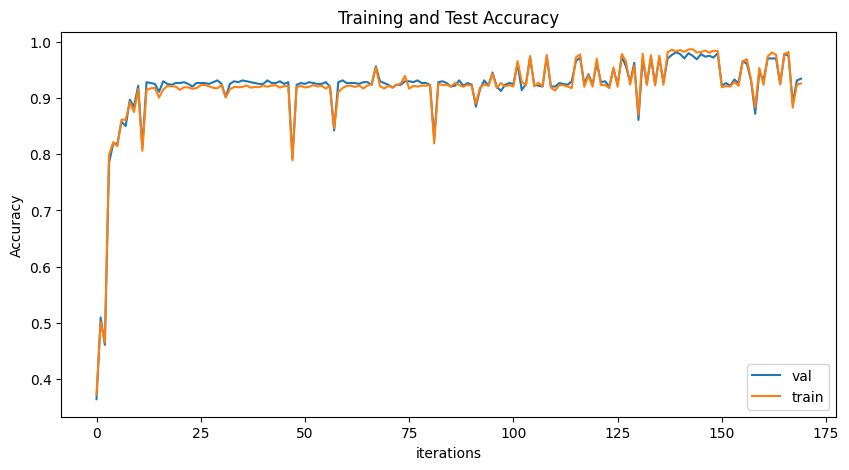
\includegraphics[width=0.8\textwidth]{images/30_results/train_test_acc.png}
    \caption{Genauigkeit des Modells während des Trainings}
    \label{fig:accuracy}
\end{figure}



\section{Testen der Hypothesen}

Im Rahmen der Arbeit werden drei Hypothesen formuliert. 
In diesem Kapitel wurden die Methoden zur Erarbeitung von Resultaten entwickelt, um diese Hypothesen zu beantworten.

Die Hypothesen lauten wie folgt:

\begin{itemize}
    \item [H1] Topologische Indizes können miteinander verglichen werden, indem sie in einer Menge $\mathcal{G}$ Graphen einer Netzwerkklasse $\mathcal{N}$ gegenübergestellt und analysiert werden.
    \item [H2] Ein nützlicher topologischer Index $\Phi$ für die Eingabe eines Netzwerkes kann gefunden werden, indem die Relevanzen der topologischen Indizes innerhalb der Netzwerkklasse $\mathcal{N}$ definiert und berechnet werden.
    \item [H3] Durch den Einsatz von Machine Learning kann der Prozess für das Analysieren und Untersuchen der Relevanz von $\Phi$ in $\mathcal{N}$ verbessert und vereinfacht werden.
\end{itemize}

\subsubsection{H1: Vergleichbarkeit der topologischen Indizes}

Zur Überprüfung von Hypothese H1 wurden die topologischen Indizes in einem oder mehreren Netzwerken verglichen. 
Hierbei wurde ein statistischer Ansatz gewählt und verschiedene Graphen mit unterschiedlichen Strukturen erzeugt. 
Die normalisierten Daten wurden visuell dargestellt und auf ihre Korrelation innerhalb der Klassen getestet. 
Es ist festzustellen, dass die topologischen Indizes miteinander verglichen werden können.

\subsubsection{H2: Berechnung des nützlichen topologischen Index}

Zur Überprüfung von Hypothese H2 wurde die PCA-Methode angewendet und die Komponenten der PCs analysiert.
Aus der Analyse der Komponenten wurde ersichtlich, dass einige topologische Indizes innerhalb der PCs mehr Aussagekraft haben als andere.
Dies bestätigt auch die Analyse der Vergleichbarkeit und Korrelation der topologischen Indizes.
Es wurde der topologische Index mit der höchsten Relevanz für die erste und zweite PC gewählt.

\subsubsection{H3: Machine Learning}

Zur Überprüfung von Hypothese H3 wurde ein GCN trainiert.
Diese hat eine Genauigkeit von über 90 \% erreicht, was bedeutet, dass es 90 \% der Graphen korrekt klassifiziert hat.
Das GCN wurde verwendet, um die Klassen der Graphen zu bestimmen.
Somit konnten die Erkenntnisse aus Hypothese H1 und H2 auf die Klassen der Graphen übertragen werden.